\documentclass[titlepage,a4paper,12pt,oneside,dvipdfmx]{jsbook}
\usepackage[dvipdfmx]{graphicx}
\usepackage{amsmath,amssymb}
\usepackage{mathrsfs}
\usepackage{amsthm}
\usepackage{booktabs}
\usepackage{bm}
\usepackage{plext}
\usepackage{color} 
\usepackage{here}
%\usepackage{slashbox}
\usepackage{comment}

%\usepackage{emathUtf}
%\usepackage{subfigure}
%\usepackage[subrefformat=parens]{subcaption}
\newtheorem{theorem}{定理}
\renewcommand{\figurename}{Fig.}
\renewcommand{\tablename}{Table }
\newcommand{\dsp}{\displaystyle}
\setlength{\textheight}{20cm}
\setlength{\textwidth}{13.5cm}
%\setlength{\textheight}{22cm}
%\setlength{\textwidth}{15cm}

\setlength{\marginparwidth}{1.5cm}


	\setlength{\topmargin}{40pt}
	\iftombow
 	\addtolentgh{\topmargin}{-1in}
	\else
 	\addtolength{\topmargin}{-1truein}
	\fi

\setlength{\oddsidemargin}{0.0cm}
\setlength{\evensidemargin}{0.0cm}

\begin{document}

\chapter{トポロジー導関数の定義}

\section{トポロジー導関数の定義}
\begin{figure}[ht]
	\begin{center}
		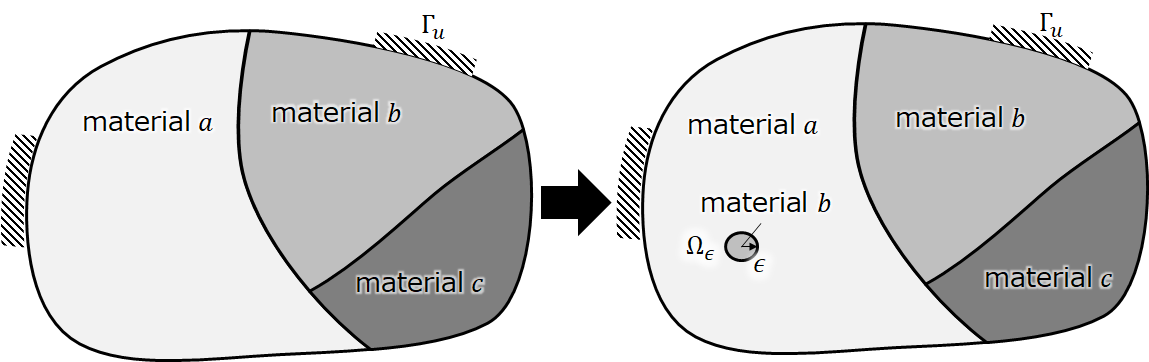
\includegraphics[width=13cm]{./figures/GeneHole.png}
		\caption{Definition of topological derivative}
		\label{fig:GeneHole}
	\end{center}
\end{figure}

トポロジー導関数は設計領域中で定義される関数で,各点$\bm{x}$を中心とする微小な円領域が,別の材料に置き換わった時の目的関数の感度を表す.
図\ref{fig:GeneHole}のように,材料$a$の占める領域中の位置$\bm{x}=\bm{z}$を中心とする微小な円領域に,材料$b$が生じた際のトポロジー導関数$D_{T}F^{a\rightarrow b}(\bm{z})$は以下のように定義される.
\begin{align}
D_{T}F^{a\rightarrow b}(\bm{z})=\lim_{\epsilon\rightarrow 0}\frac{\delta F^{a\rightarrow b}(\bm{z})}{g(\epsilon)}
\end{align}
ここで,$\delta F^{a\rightarrow b}$は目的関数の変化,$g(\epsilon)$は極限値が存在するように定義される$\epsilon$の関数である.
一般的に次式のように$\Omega_{\epsilon}$の測度で定義される.
\begin{align}
g(\epsilon)=&\pi\epsilon^2 \hspace{1cm}\text{(for 2D)} \\
=&\frac{3}{4}\pi\epsilon^3 \hspace{0.8cm}\text{(for 3D)}
\end{align}

\section{Topological-Shape Sensitivity Method}

\begin{figure}[ht]
	\begin{center}
		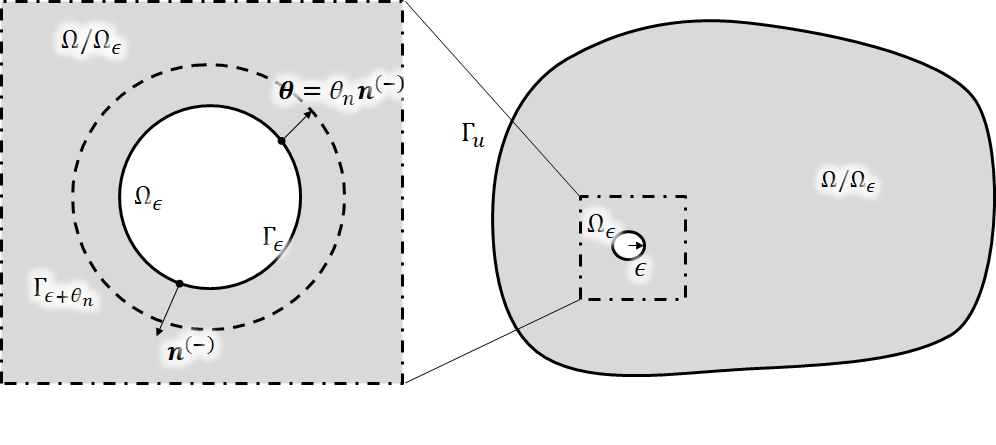
\includegraphics[width=13cm]{./figures/TSSM.png}
		\caption{Concept of Topological-Shape Sensitivity Method}
		\label{fig:TSSM}
	\end{center}
\end{figure}

Novotny et al.は形状微分の極限をとることでトポロジー導関数を導出する方法を提案した.
形状微分とは構造の境界が微小量移動した時の目的関数の感度である.

$\bm{\theta}(\bm{x})$方向に形状が微小変動するとき,領域写像$\psi_{s}(\bm{x})$は次式のように表される.
\begin{align}
\psi_{s}(\bm{x})=\bm{x}+s\bm{\theta}(\bm{x})
\end{align}
この時,形状微分$DF(\Omega)\cdot\bm{\theta}$は以下のように定義される.
\begin{align}
DF(\Omega)\cdot\bm{\theta}=\frac{d}{ds}F(\psi_{s}(\Omega))
\end{align}
図\ref{fig:TSSM}のように半径$\epsilon$の空洞$\Omega_{\epsilon}$が物体領域$\Omega/\Omega_{\epsilon}$内向き法線$\bm{n}^{(-)}$方向に膨張する時,つまり
\begin{align}
\bm{\theta}=&\theta_{n}\bm{n}^{(-)}	\hspace{1cm}\text{on}\hspace{0.3cm}\Gamma_{\epsilon}\\
\bm{\theta}=&\bm{0}					\hspace{1.8cm}\text{on}\hspace{0.3cm}\Gamma/\Gamma_{\epsilon}
\end{align}
となる時の形状微分を考える.$\theta_{n}$は正の値をとる定数である.
トポロジー導関数は以下のように$\epsilon\rightarrow0$の極限をとることで得られる.
\begin{align}
D_{T}F=\lim_{\epsilon\rightarrow 0}\frac{1}{g'(\epsilon)|\theta_{n}|}\Bigl(DF\cdot \bm{\theta}\Bigr)(\epsilon)
\label{eq:TSSen}
\end{align}
ただし,$g'(\epsilon)$は$g(\epsilon)$の$\epsilon$に関する微分を表す.
このような,形状微分に基づくトポロジー導関数の導出方法をTopological-Shape Sensitivity Methodと呼び,
以下のプロセスで導出する.
まず,形状微分$DF\cdot \bm{\theta}$を求める.
次に,$\epsilon\rightarrow0$とした時の状態場や随伴場の漸近的な振る舞いを調べる.
その結果を式\eqref{eq:TSSen}に代入することでトポロジー導関数を導出する.


\chapter{弾性体の固有振動問題}

\section{固有振動問題の支配方程式}
最大$n$個の材料を用いる場合を考える.
$p$番目$(1\leq p\leq n)$の材料が占める領域を$\Omega_{p}$,
$p$番目の材料と$q$番目の材料の境界を$\Gamma_{pq}$とする.
固有値$\lambda$とそれに対応する固有振動モード$\bm{u}$は以下の支配方程式に従う.
\begin{align}
	&C_{ijkl}^{p}u_{k,lj}^{}+\lambda\rho^{p} u_{i}=0&\text{in}\hspace{0.3cm}\Omega_{p}
	\label{eq:govmain}
	\\
	&u_{i}=0 &\text{on}\hspace{0.3cm}\Gamma_{D}
	\\
	&C_{ijkl}u_{k,l}^{}n_{j}=0 &\text{on}\hspace{0.3cm}\Gamma_{N}
	\\
	&u_{i}^{p}=u_{i}^{p} &\text{on}\hspace{0.3cm}\Gamma_{pq}
	\\
	&C_{ijkl}^{p}u_{k,l}^{p}n_{j}^{p}+C_{ijkl}^{q}u_{k,l}^{q}n_{j}^{q}=0 &\text{on}\hspace{0.3cm}\Gamma_{pq}
	\label{eq:govbc}
	\\
	&\sum_{p=1}^{n}\int_{\Omega_p}(\rho^{p}u_{i}u_{i}) d\Omega=1
	\label{eq:govnorm}
\end{align}
ただし,$C_{ijkl}$は弾性テンソル,$\rho$は質量密度を表す.

\section{固有振動数最大化問題の目的関数}

1番目から$\alpha$番目までの固有振動数の最大化を目的とする場合,目的関数は以下のように,$\alpha$番目までの固有値の調和平均の形で定義される.
\begin{align}
\min_{\Omega_{p}\{1\leq p\leq n\}}F=-\Bigr(\sum_{\beta=1}^{\alpha}\frac{1}{\lambda_{\beta}}\Bigl)^{-1}
\end{align}
ただし,$\lambda_{\beta}$は$\beta$番目の固有値を表す.$\alpha$個の固有値の内,小さいものから順に目的関数への影響が大きいため,この目的関数を最小化することで小さい固有値から優先的に最大化される.

この目的関数のトポロジー導関数は連鎖率から以下のように表される.
\begin{align}
D_{T}F	=&\sum_{\beta=1}^{\alpha}\frac{\partial F}{\partial \lambda_{\beta}}D_{T}\lambda_{\beta}
		\nonumber
		\\
		=&-\Bigr(\sum_{\beta=1}^{\alpha}\frac{1}{\lambda_{\beta}}\Bigl)^{-2}
		\Bigr(\sum_{\beta=1}^{\alpha}\frac{D_{T}\lambda_{\beta}}{\lambda_{\beta}^2}\Bigl)
\end{align}
ゆえに,固有値$\lambda$のトポロジー導関数を導出することで,目的関数のトポロジー導関数が得られる.


\chapter{形状微分}
\section{形状微分の公式}

\begin{figure}[ht]
	\begin{center}
		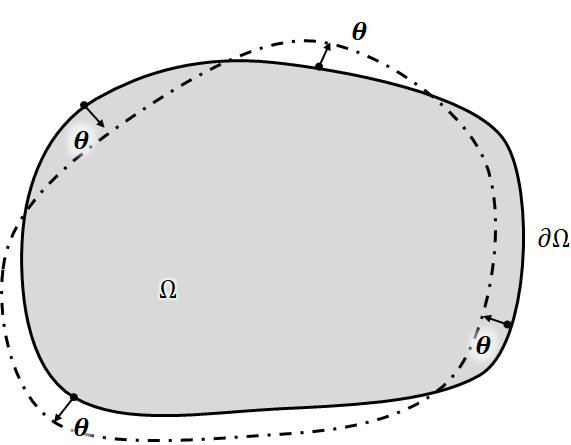
\includegraphics[height=5cm]{./figures/SDFormula.png}
		\caption{Deformation in $\bm{\theta}$ direction}
		\label{fig:SDFormula}
	\end{center}
\end{figure}

形状微分には以下のような公式が存在する.

汎関数$J$が積分領域$\Omega$に依存しない密度関数$f$の領域積分によって,次式のように表されるとする.
\begin{align}
	J=\int_{\Omega}f d\Omega
	\label{eq:functinal_d}
\end{align}
この時,$J$の形状微分は次式で得られる.
\begin{align}
	DJ\cdot\theta=\int_{\Gamma}(\theta_{i}n_{i})f d\Omega
	\label{eq:drivative_d}
\end{align}
ただし,$\bm{n}$は$\Gamma$上の外向きの単位法線ベクトルを表す.

次に,汎関数$J$が密度関数$f$の境界積分によって,次式のように表される場合を考える.
\begin{align}
	J=\int_{\Gamma}f d\Gamma
	\label{eq:functinal_b}
\end{align}
この時,$J$の形状微分は次式で得られる.
\begin{align}
	DJ\cdot\theta=\int_{\Gamma}(\theta_{i}n_{i})\Bigr(\frac{\partial f}{\partial x_{j}}n_{j}+Hf\Bigl) d\Omega
	\label{eq:drivative_b}
\end{align}
ただし,$H\equiv div\bm{n}$は$\Gamma$の平均曲率を表す.

公式\eqref{eq:drivative_d},\eqref{eq:drivative_b}はいずれも密度関数$f$が積分領域に依存しないことが条件であることに注意が必要である.

\section{ラグラジアンの定式化}

\begin{figure}[ht]
	\begin{center}
		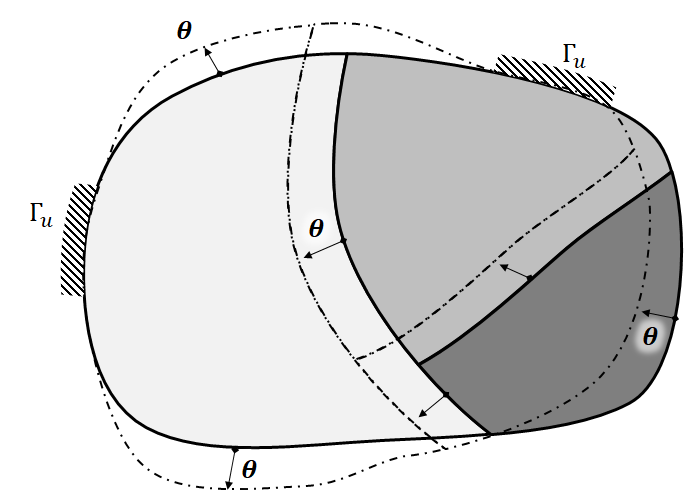
\includegraphics[height=5cm]{./figures/SD.png}
		\caption{Shape derivative}
		\label{fig:SD}
	\end{center}
\end{figure}

ラグラジアンを以下のように定式化する.
\begin{align}
	\mathscr{L}(\Omega_{p\{1\leq p\leq n\}};\bm{U},X,\bm{V},Y)=
	&X+\sum_{p=1}^{n}\int_{\Omega_p}\Bigr( V_{i,j}C_{ijkl}^{p}U_{k,l}-X\rho^{p}V_{i}U_{i}\Bigl) d\Omega
	\nonumber
	\\
	&-\sum_{p=1}^{n-1}\sum_{p=q}^{n}\int_{\Gamma_{pq}}\frac{1}{2}\Bigr(C_{ijkl}^{p}U_{k,l}^{p}n_{j}^{p}-C_{ijkl}^{q}U_{k,l}^{q}n_{j}^{q}\Bigl)(V_{i}^{p}-V_{i}^{q}) d\Gamma
	\nonumber
	\\
	&-\sum_{p=1}^{n-1}\sum_{p=q}^{n}\int_{\Gamma_{pq}}\frac{1}{2}\Bigr(V_{i,j}^{p}C_{ijkl}^{p}n_{l}^{p}-V_{i,j}^{q}C_{ijkl}^{q}n_{l}^{q}\Bigl)(U_{k}^{p}-U_{k}^{q})d\Gamma
	\nonumber
	\\
	&-\sum_{p=1}^{n}\int_{\Gamma_{pu}}\Bigr(C_{ijkl}^{p}U_{k,l}^{p}n_{j}^{p}\Bigl)(V_{i}^{p}) d\Gamma
	\nonumber
	\\
	&-\sum_{p=1}^{n}\int_{\Gamma_{pu}}\Bigr(V_{i,j}^{p}C_{ijkl}^{p}n_{l}^{p}\Bigl)(U_{k}^{p}) d\Gamma
	\nonumber
	\\
	&+Y\Bigr\{1- \sum_{p=1}^{n}\int_{\Omega_{p}}(\rho^{p}U_{i}U_{i}) d\Omega \Bigl\}
	\label{eq:lagrange}
\end{align}
$\bm{U},X$はそれぞれ状態変数$\bm{u},\lambda$に対応する変数,$\bm{V},Y$はラグランジュ乗数である.
ここで,$\bm{u}$や$\lambda$が領域$\Omega_p$に依存する関数であるのに対し,$\bm{U},X,\bm{V},Y$は$\Omega_p$に依存しない関数であることに注意が必要である.

ラグラジアン\eqref{eq:lagrange}に対し,$\bm{V}$に関して部分積分を行うと
\begin{align}
	\mathscr{L}(\Omega_{p\{1\leq p\leq n\}};\bm{U},X,\bm{V},Y)=&X-\sum_{p=1}^{n}\int_{\Omega_p}\Bigr(C_{ijkl}^{p}U_{k,lj}+X\rho^{p}U_{i}\Bigl)V_{i} d\Omega
	\nonumber
	\\
	&+\sum_{p=1}^{n-1}\sum_{p=q}^{n}\int_{\Gamma_{pq}}\frac{1}{2}\Bigr(C_{ijkl}^{p}U_{k,l}^{p}n_{j}^{p}+C_{ijkl}^{q}U_{k,l}^{q}n_{j}^{q}\Bigl)(V_{i}^{p}-V_{i}^{q}) d\Gamma
	\nonumber
	\\
	&-\sum_{p=1}^{n-1}\sum_{p=q}^{n}\int_{\Gamma_{pq}}\frac{1}{2}\Bigr(V_{i,j}^{p}C_{ijkl}^{p}n_{l}^{p}-V_{i,j}^{q}C_{ijkl}^{q}n_{l}^{q}\Bigl)(U_{k}^{p}-U_{k}^{q})d\Gamma
	\nonumber
	\\
	&+\sum_{p=1}^{n}\int_{\Gamma_{pN}}\Bigr(C_{ijkl}^{p}U_{k,l}^{p}n_{j}^{p}\Bigl)(V_{i}^{p}) d\Gamma
	\nonumber
	\\
	&-\sum_{p=1}^{n}\int_{\Gamma_{pu}}\Bigr(V_{i,j}^{p}C_{ijkl}^{p}n_{l}^{p}\Bigl)(U_{k}^{p}) d\Gamma
	\nonumber
	\\
	&+Y\Bigr\{1- \sum_{p=1}^{n}\int_{\Omega_{p}}(\rho^{p}U_{i}U_{i}) d\Omega \Bigl\}
	\nonumber
	\\
	\label{eq:lagrange_vint}
\end{align}
状態方程式\eqref{eq:govmain}~\eqref{eq:govnorm}より,$\bm{U}=\bm{u}(\Omega_{p\{1\leq p\leq n\}})$,
$X=\lambda(\Omega_{p\{1\leq p\leq n\}})$とすれば,任意の$\bm{V},Y$に対して次式が成立することがわかる.
\begin{align}
	\mathscr{L}(\Omega_{p\{1\leq p\leq n\}};\bm{u},\lambda,\bm{U},Y)=\lambda(\Omega_{p\{1\leq p\leq n\}})
	\label{eq:Lagrange_lambda}
\end{align}

\section{ラグラジアンの停留条件}

式\eqref{eq:Lagrange_lambda}より,$\lambda(\Omega_{p\{1\leq p\leq n\}})$の形状微分は次式のように表される.
\begin{align}
	D\lambda(\Omega_{p\{1\leq p\leq n\}})\cdot\bm{\theta}
	=&D\mathscr{L}(\Omega_{p\{1\leq p\leq n\}};\bm{u},\lambda,\bm{V},Y)\cdot\bm{\theta}
	\nonumber
	\\
	&+\Bigr\langle \frac{\partial \mathscr{L}}{\partial \bm{V}}(\Omega_{p\{1\leq p\leq n\}};\bm{u},\lambda,\bm{V},Y),
	\delta\bm{u} \Bigl\rangle
	\nonumber
	\\
	&+\frac{\partial \mathscr{L}}{\partial X}(\Omega_{p\{1\leq p\leq n\}};\bm{u},\lambda,\bm{V},Y)\cdot
	\delta\lambda
	\label{eq:shape_lagrange}
\end{align}
ここで,$\delta\bm{u}$および$\delta\lambda$はそれぞれ状態場$\bm{u}$および$\lambda$の変分である.
$\bm{u}$および$\lambda$が状態方程式を介して領域$\Omega_{p}$に依存しているため,連鎖率によって上式の右辺第2項および第3項が生じている.
しかし,$\delta\bm{u}$および$\delta\lambda$は導出することが困難であるため,
それらの計算を回避するためにラグラジアンの停留条件を考える.
\begin{align}
	\left.\bigr\langle \frac{\partial \mathscr{L}}{\partial \bm{U}},\delta \bm{U} \bigl\rangle\right|_{opt}=0
	\label{eq:optc_u}
	\\
	\left.\frac{\partial\mathscr{L}}{\partial X}\right|_{opt}=0
	\label{eq:optc_x}
	\\
	\left.\bigr\langle \frac{\partial \mathscr{L}}{\partial \bm{V}},\delta \bm{V} \bigl\rangle\right|_{opt}=0
	\label{eq:optc_v}
	\\
	\left.\frac{\partial\mathscr{L}}{\partial Y}\right|_{opt}=0
	\label{eq:optc_y}
\end{align}
まず,式\eqref{eq:optc_v},\eqref{eq:optc_y}に関しては,式\eqref{eq:lagrange_vint}より次式のようになる.
\begin{align}
	0=&\left.\bigr\langle \frac{\partial \mathscr{L}}{\partial \bm{V}},\delta \bm{V} \bigl\rangle\right|_{opt}
	\nonumber
	\\
	=&\sum_{p=1}^{n}\int_{\Omega_p}\Bigr(C_{ijkl}^{p}U_{k,lj}+X\rho^{p}U_{i}\Bigl)\delta V_{i} d\Omega
	\nonumber
	\\
	&+\sum_{p=1}^{n-1}\sum_{p=q}^{n}\int_{\Gamma_{pq}}\frac{1}{2}\Bigr(C_{ijkl}^{p}U_{k,l}^{p}n_{j}^{p}+C_{ijkl}^{q}U_{k,l}^{q}n_{j}^{q}\Bigl)(\delta V_{i}^{p}-\delta V_{i}^{q}) d\Gamma
	\nonumber
	\\
	&-\sum_{p=1}^{n-1}\sum_{p=q}^{n}\int_{\Gamma_{pq}}\frac{1}{2}\Bigr(\delta V_{i,j}^{p}C_{ijkl}^{p}n_{l}^{p}-\delta V_{i,j}^{q}C_{ijkl}^{q}n_{l}^{q}\Bigl)(U_{k}^{p}-U_{k}^{q})d\Gamma
	\nonumber
	\\
	&+\sum_{p=1}^{n}\int_{\Gamma_{pN}}\Bigr(U_{i,j}^{p}C_{ijkl}^{p}n_{l}^{p}\Bigl)(\delta V_{i}^{p}) d\Gamma
	\nonumber
	\\
	&-\sum_{p=1}^{n}\int_{\Gamma_{pu}}\Bigr(\delta V_{i,j}^{p}C_{ijkl}^{p}n_{l}^{p}\Bigl)(U_{k}^{p}) d\Gamma
	\label{eq:lagrange_vderivative}
\end{align}
\begin{align}
	0=\left.\frac{\partial \mathscr{L}}{\partial Y}\right|_{opt}=1- \sum_{p=1}^{n}\int_{\Omega_{p}}(\rho^{p}U_{i}U_{i}) d\Omega
	\label{eq:lagrange_yderivative}
\end{align}
上式と状態方程式\eqref{eq:govmain}~\eqref{eq:govnorm}との比較から,$\bm{U}=\bm{u}(\Omega_{p\{1\leq p\leq n\}})$,$X=\lambda(\Omega_{p\{1\leq p\leq n\}})$の時,
任意の$\delta \bm{V}$に対して停留条件\eqref{eq:optc_v},\eqref{eq:optc_y}が成立することがわかる.

$\bm{V}=\bm{v}(\Omega_{p\{1\leq p\leq n\}}),Y=\eta(\Omega_{p\{1\leq p\leq n\}})$が$\bm{U},X$に関する停留条件\eqref{eq:optc_u},\eqref{eq:optc_x}
を満たすとすると,$\lambda$の形状微分は以下のように表される.
\begin{align}
	D\lambda(\Omega_{p\{1\leq p\leq n\}})\cdot\bm{\theta}
	=&D\mathscr{L}(\Omega_{p\{1\leq p\leq n\}};\bm{u},\lambda,\bm{v},\eta)\cdot\bm{\theta}
	\nonumber
	\\
	&+\Bigr\langle \frac{\partial \mathscr{L}}{\partial \bm{U}}(\Omega_{p\{1\leq p\leq n\}};\bm{u},\lambda,\bm{v},\eta),
	\delta\bm{u} \Bigl\rangle
	\nonumber
	\\
	&+\frac{\partial \mathscr{L}}{\partial X}(\Omega_{p\{1\leq p\leq n\}};\bm{p},\lambda,\bm{v},\eta)\cdot
	\delta\lambda
	\nonumber
	\\
	&+\Bigr\langle \frac{\partial \mathscr{L}}{\partial \bm{V}}(\Omega_{p\{1\leq p\leq n\}};\bm{u},\lambda,\bm{v},\eta),
	\delta\bm{v} \Bigl\rangle
	\nonumber
	\\
	&+\frac{\partial \mathscr{L}}{\partial Y}(\Omega_{p\{1\leq p\leq n\}};\bm{p},\lambda,\bm{v},\eta)\cdot
	\delta\eta
	\nonumber
	\\
	=&D\mathscr{L}(\Omega_{p\{1\leq p\leq n\}};\bm{u},\lambda,\bm{v},\eta)\cdot\bm{\theta}
	\label{eq:shape_lambda_uv}
\end{align}
ここで,上式の中辺第2項から第5項が停留条件\eqref{eq:optc_u}~\eqref{eq:optc_y}より,
任意の$\delta\bm{u},\delta\lambda,\delta\bm{v},\delta\eta$に対して0になることを用いた.
式\eqref{eq:shape_lambda_uv}より,ラグラジアンの形状微分の式に$\bm{U}=\bm{u},X=\lambda,\bm{V}=\bm{v},Y=\eta$
を代入することで,固有値$\lambda$の形状微分が得られることが分かる.

\section{随伴方程式}
続いて,$\bm{U},X$に関する停留条件\eqref{eq:optc_u},\eqref{eq:optc_x}をみたすような,
$\bm{V}=\bm{v}(\Omega_{p\{1\leq p\leq n\}}),Y=\eta(\Omega_{p\{1\leq p\leq n\}})$の条件について考える.

ラグラジアン\eqref{eq:lagrange}に対し,$\bm{U}$に関して部分積分を行うと
\begin{align}
	\mathscr{L}(\Omega_{p\{1\leq p\leq n\}};\bm{U},X,\bm{V},Y)=&X-\sum_{p=1}^{n}\int_{\Omega_p}\Bigr(V_{i,jl}C_{ijkl}^{p}+X\rho^{p}V_{k}\Bigl)U_{k} d\Omega
	\nonumber
	\\
	&-\sum_{p=1}^{n-1}\sum_{p=q}^{n}\int_{\Gamma_{pq}}\frac{1}{2}\Bigr(C_{ijkl}^{p}U_{k,l}^{p}n_{j}^{p}-C_{ijkl}^{q}U_{k,l}^{q}n_{j}^{q}\Bigl)(V_{i}^{p}-V_{i}^{q}) d\Gamma
	\nonumber
	\\
	&+\sum_{p=1}^{n-1}\sum_{p=q}^{n}\int_{\Gamma_{pq}}\frac{1}{2}\Bigr(V_{i,j}^{p}C_{ijkl}^{p}n_{l}^{p}+V_{i,j}^{q}C_{ijkl}^{q}n_{l}^{q}\Bigl)(U_{k}^{p}-U_{k}^{q})d\Gamma
	\nonumber
	\\
	&+\sum_{p=1}^{n}\int_{\Gamma_{pN}}\Bigr(V_{i,j}^{p}C_{ijkl}^{p}n_{l}^{p}\Bigl)(U_{k}^{p}) d\Gamma
	\nonumber
	\\
	&-\sum_{p=1}^{n}\int_{\Gamma_{pu}}\Bigr(C_{ijkl}^{p}U_{k,l}^{p}n_{j}^{p}\Bigl)(V_{i}^{p}) d\Gamma
	\nonumber
	\\
	&+Y\Bigr\{1- \sum_{p=1}^{n}\int_{\Omega_{p}}(\rho^{p}U_{i}U_{i}) d\Omega \Bigl\}
	\nonumber
	\\
	\label{eq:lagrange_uint}
\end{align}
となるため,停留点における$\bm{V}$および$Y$をそれぞれ$\bm{v}$,$\eta$とすると,式\eqref{eq:optc_u},\eqref{eq:optc_x}は以下のようになる.
\begin{align}
	0=&\left.\bigr\langle \frac{\partial \mathscr{L}}{\partial \bm{U}},\delta \bm{U} \bigl\rangle\right|_{opt}
	\nonumber
	\\
	=&\sum_{p=1}^{n}\int_{\Omega_p}\Bigr(v_{k,lj}C_{ijkl}^{p}+\lambda\rho^{p}v_{i}+2\eta\rho^{p}u_{i}\Bigl)\delta U_{i} d\Omega
	\nonumber
	\\
	&-\sum_{p=1}^{n-1}\sum_{p=q}^{n}\int_{\Gamma_{pq}}\frac{1}{2}\Bigr(\delta U_{i,j}^{p}C_{ijkl}^{p}n_{l}^{p}-\delta U_{i,j}^{q}C_{ijkl}^{q}n_{l}^{q}\Bigl)(v_{k}^{p}-v_{k}^{q}) d\Gamma
	\nonumber
	\\
	&+\sum_{p=1}^{n-1}\sum_{p=q}^{n}\int_{\Gamma_{pq}}\frac{1}{2}\Bigr(v_{k,l}^{p}C_{ijkl}^{p}n_{j}^{p}+v_{k,l}^{q}C_{ijkl}^{q}n_{j}^{q}\Bigl)(\delta U_{i}^{p}-\delta U_{i}^{q})d\Gamma
	\nonumber
	\\
	&+\sum_{p=1}^{n}\int_{\Gamma_{pN}}\Bigr(v_{k,l}^{p}C_{ijkl}^{p}n_{j}^{p}\Bigl)\delta U_{i}^{p} d\Gamma
	\nonumber
	\\
	&-\sum_{p=1}^{n}\int_{\Gamma_{pu}}\Bigr(\delta U_{i,j}^{p}C_{ijkl}^{p}n_{l}^{p}\Bigl)v_{k}^{p} d\Gamma
	\label{eq:lagrange_uderivative}
\end{align}
\begin{align}
	0=\left.\frac{\partial\mathscr{L}}{\partial X}\right|_{opt}
	=1-\sum_{p=1}^{n}\int_{\Omega_p}\bigr(\rho^{p}v_{i}u_{i}\bigl) d\Omega
	\label{eq:lagrange_xderivative}
\end{align}
ここで,$C_{ijkl}=C_{klij}$であることを用いて,添え字を$(i,j,k,l)\rightarrow(k,l,i,j)$に変換した.
以上から,$\bm{v}$,$\eta$が以下の随伴方程式を満たすとき,停留条件\eqref{eq:optc_u},\eqref{eq:optc_x}は成立する.
\begin{align}
	&C_{ijkl}^{p}v_{k,lj}+\lambda\rho^{p}v_{i}+2\eta\rho^{p} u_{i}=0&\text{in}\hspace{0.3cm}\Omega_{p}
	\label{eq:adjmain}
	\\
	&v_{i}=0 &\text{on}\hspace{0.3cm}\Gamma_{D}
	\\
	&C_{ijkl}v_{k,l}^{}n_{j}=0 &\text{on}\hspace{0.3cm}\Gamma_{N}
	\\
	&v_{i}^{p}=v_{i}^{q} &\text{on}\hspace{0.3cm}\Gamma_{pq}
	\\
	&C_{ijkl}^{p}v_{k,l}^{p}n_{j}^{p}+C_{ijkl}^{q}v_{k,l}^{q}n_{j}^{q}=0 &\text{on}\hspace{0.3cm}\Gamma_{pq}
	\label{eq:adjbc}
	\\
	&\sum_{p=1}^{n}\int_{\Omega_p}(\rho^{p}v_{i}u_{i}) d\Omega=1
	\label{eq:adjnorm}
\end{align}
次に,$\eta$の値を求める.
まず,強形式の状態方程式\eqref{eq:govmain}に$\bm{v}$をかけ,領域積分することで次式が得られる.
\begin{align}
	\sum_{p=1}^{n}\int_{\Omega_p}\Bigr(v_{i,j}C_{ijkl}^{p}u_{k,l}-\lambda\rho^{p}v_{i}u_{i}\Bigl) d\Omega=0
	\label{eq:gov_p}
\end{align}
強形式の随伴方程式\eqref{eq:adjmain}に$\bm{u}$をかけ,領域積分することで次式が得られる.
\begin{align}
	\sum_{p=1}^{n}\int_{\Omega_p}\Bigr(v_{i,j}C_{ijkl}^{p}u_{k,l}-\lambda\rho^{p}u_{i}^{}v_{i}^{}-2\eta u_{i}^{}u_{i}^{}\Bigl) d\Omega=0
	\label{eq:adj_u}
\end{align}
式\eqref{eq:gov_p}と式\eqref{eq:adj_u}の差を取り,正規化条件\eqref{eq:govnorm}を用いることで以下のように$\eta$が求まる.
\begin{align}
	\eta\sum_{p=1}^{n}\int_{\Omega_p}(\rho^{p}u_{i}^{}u_{i}^{}) d\Omega=\eta=0
	\label{eq:eta_0}
\end{align}
ゆえに,随伴場の偏微分方程式\eqref{eq:adjmain}~\eqref{eq:adjbc}は状態場の偏微分方程式\eqref{eq:govmain}~\eqref{eq:govbc}と等しくなり,
随伴場$\bm{v}$は次式のように状態場$\bm{u}$の定数倍で与えられる.
\begin{align}
	\bm{v}=K\bm{u}
	\label{eq:v_ku}
\end{align}
さらに,状態場と随伴場の正規化条件\eqref{eq:govnorm},\eqref{eq:adjnorm}より,次式のようにKの値が求まる.
\begin{align}
	1&=\sum_{p=1}^{n}\int_{\Omega_p}\Bigr(\rho^{p}u_{i}v_{i}\Bigl) d\Omega
	\nonumber
	\\
	&=K\sum_{p=1}^{n}\int_{\Omega_p}\Bigr(\rho^{p}u_{i}u_{i}\Bigl) d\Omega
	\nonumber
	\\
	&=K
	\label{eq:k}
\end{align}
ゆえに,$\bm{u}$と$\bm{v}$は等しい.
\begin{align}
	\bm{v}=\bm{u}
	\label{eq:v_u}
\end{align}

\section{形状微分の公式の適用}

式\eqref{eq:shape_lambda_uv}に式\eqref{eq:eta_0},\eqref{eq:v_u}を代入することで,
固有値$\lambda$の形状微分は次式のように表される.
\begin{align}
	D\lambda\cdot\bm{\theta}
	=&D\mathscr{L}(\Omega_{p\{1\leq p\leq n\}};\bm{u},\lambda,\bm{u},0)\cdot\bm{\theta}
	\label{eq:shape_lambda_u}
\end{align}

形状微分の公式\eqref{eq:drivative_d},\eqref{eq:drivative_b}を式\eqref{eq:shape_lambda_u}のラグラジアンの形状微分に適用し,
$\Gamma_{u}$上で$\bm{\theta}=\bm{0}$を仮定すると次式が得られる.
\begin{align}
	&\hspace{0.5cm}D\lambda\cdot\bm{\theta}
	\nonumber
	\\
	&=D\mathscr{L}(\Omega_{p\{1\leq p\leq n\}};\bm{u},\lambda,\bm{u},0)\cdot\bm{\theta}
	\nonumber
	\\
	&=\sum_{p=1}^{n}\int_{\Gamma_p}(\theta_{m}n_{m}^{p})\Bigr(u_{i,j}C_{ijkl}^{p}u_{k,l}-\lambda\rho^{p}u_{i}u_{i}\Bigl) d\Omega
	\nonumber
	\\
	&-\sum_{p=1}^{n-1}\sum_{p=q}^{n}\int_{\Gamma_{pq}}(\theta_{m}n_{m}^{p})
	\Bigr(\frac{\partial}{\partial x_\gamma }n_\gamma^{p} +H^{p}\Bigl)
	\Bigr(C_{ijkl}^{p}u_{k,l}^{p}n_{j}^{p}-C_{ijkl}^{q}u_{k,l}^{q}n_{j}^{q}\Bigl)
	(u_{i}^{p}-u_{i}^{q}) d\Gamma
	\label{eq:shape_lambda}
\end{align}
境界条件から$\partial \Omega_{pq}$上で$\bm{u}^{p}=\bm{u}^{q}$であることに注意すると,
固有値$\lambda$の形状微分は次式のように導出される.
\begin{align}
	\hspace{0.5cm}D\lambda\cdot\bm{\theta}
	=&\sum_{p=1}^{n}\int_{\Gamma_p}(\theta_{m}n_{m}^{p})\Bigr(u_{i,j}C_{ijkl}^{p}u_{k,l}-\lambda\rho^{p}u_{i}u_{i}\Bigl) d\Omega
	\nonumber
	\\
	&-\sum_{p=1}^{n-1}\sum_{p=q}^{n}\int_{\Gamma_{pq}}(\theta_{m}n_{m}^{p})
	\Bigr(C_{ijkl}^{p}u_{k,l}^{p}n_{j}^{p}-C_{ijkl}^{q}u_{k,l}^{q}n_{j}^{q}\Bigl)
	(u_{i,\gamma}^{p}n_\gamma^{p}-u_{i,\gamma}^{q}n_\gamma^{p}) d\Gamma
	\label{eq:shape_lambda}
\end{align}




\chapter{固有振動モードの漸近展開}
\section{固有振動モードの変動に関する方程式}
\begin{figure}[ht]
	\begin{center}
		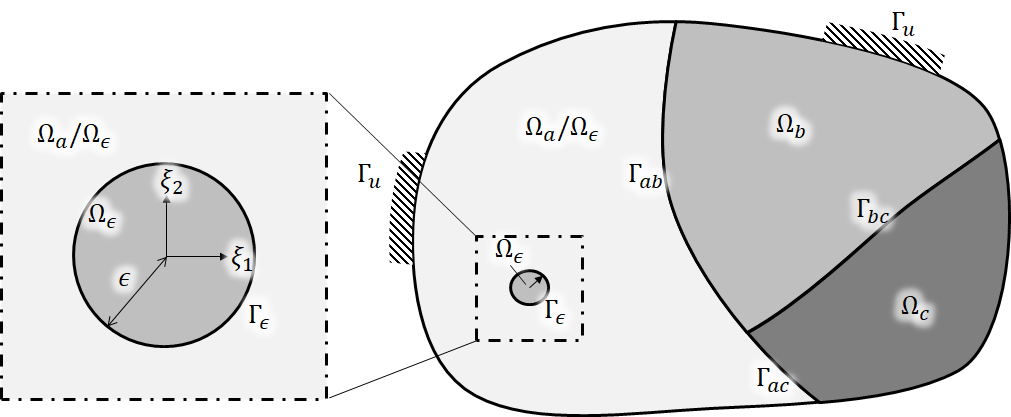
\includegraphics[width=13cm]{./figures/TD.png}
		\caption{Emergence of a circular region}
		\label{fig:TD}
	\end{center}
\end{figure}
材料$a$で占められた領域$\Omega_a$中の微小な円領域$\Omega_\epsilon$に材料$b$が生成した際の,固有振動モード$\bm{u}^{\epsilon}$および固有値$\lambda^{\epsilon}$について考える.
ただし,これによって固有振動モードの順番の変化は起こらないと仮定する.
この時の支配方程式は以下のようになる.
\begin{align}
	&C_{ijkl}^{b}u_{k,lj}^{\epsilon}+\lambda^{\epsilon}\rho^{b} u_{i}^{\epsilon}=0&&\text{in}\hspace{0.3cm}\Omega_{\epsilon}
	\label{eq:govepmain}
	\\
	&C_{ijkl}^{a}u_{k,lj}^{\epsilon}+\lambda^{\epsilon}\rho^{a} u_{i}^{\epsilon}=0&&\text{in}\hspace{0.3cm}\Omega_{a}\backslash\Omega_{\epsilon}
	\label{eq:govepmain}
	\\
	&C_{ijkl}^{p}u_{k,lj}^{\epsilon}+\lambda^{\epsilon}\rho^{p} u_{i}^{\epsilon}=0&&\text{in}\hspace{0.3cm}\Omega_{p}\hspace{0.3cm}(p\neq a)
	\label{eq:govepmain}
	\\
	&u_{i}^{\epsilon b}=u_{i}^{\epsilon a} &&\text{on}\hspace{0.3cm}\Gamma_{\epsilon}
	\\
	&C_{ijkl}^{b}u_{k,l}^{\epsilon b}n_{j}^{b}+C_{ijkl}^{a}u_{k,l}^{\epsilon a}n_{j}^{a}=0 &&\text{on}\hspace{0.3cm}\Gamma_{\epsilon}
	\label{eq:govepbc}
	\\
	&u_{i}^{\epsilon p}=u_{i}^{\epsilon q} &&\text{on}\hspace{0.3cm}\Gamma_{pq}
	\\
	&C_{ijkl}^{p}u_{k,l}^{\epsilon p}n_{j}^{p}+C_{ijkl}^{q}u_{k,l}^{\epsilon q}n_{j}^{q}=0 &&\text{on}\hspace{0.3cm}\Gamma_{pq}
	\label{eq:govepbc}
	\\
	&\sum_{p=1,p\neq a}^{n}\int_{\Omega_p}(\rho^{p}u_{i}^{\epsilon}u_{i}^{\epsilon}) d\Omega
	+\int_{\Omega_a\backslash\Omega_{\epsilon}}(\rho^{a}u_{i}^{\epsilon}u_{i}^{\epsilon}) d\Omega
	+\int_{\Omega_{\epsilon}}(\rho^{b}u_{i}^{\epsilon}u_{i}^{\epsilon}) d\Omega=1
	\label{eq:govepnorm}
\end{align}

$\bm{u}^{\epsilon},\lambda^{\epsilon}$を,微小な材料$b$の領域が生成される前の固有ベクトルおよび固有値$\bm{u},\lambda$用いて展開すると,次式のようになる.
\begin{align}
	\bm{u}^{\epsilon}(\bm{x})=&\bm{u}(\bm{x})\chi_{R^2/\Omega}+\hat{\bm{u}}(\bm{x})
	\\
	\lambda^{\epsilon}=&\lambda+\hat{\lambda}
\end{align}
ここで,$\Omega_\epsilon$の中心座標を$\bm{x}_0$とし,$\bm{\xi}=\dsp\frac{\bm{x}-\bm{z}}{\epsilon}$を導入し,
$\hat{\bm{u}}(\bm{x})$を$\epsilon$に関して次式のように漸近展開する.
\begin{align}
	\hat{\bm{u}}(\bm{x})
	=&\{\hat{\bm{u}}^{(I-)}(\bm{x})+\epsilon\hat{\bm{u}}^{(I\hspace{-.1em}I-)}(\bm{x})\}\chi_{\Omega_\epsilon}
	+\{\hat{\bm{u}}^{(I+)}(\bm{x})+\epsilon\hat{\bm{u}}^{(I\hspace{-.2em}I+)}(\bm{x})\}\chi_{R^2\backslash\Omega_\epsilon}+O(\epsilon^2)
	\nonumber
	\\
	=&\{\hat{\bm{w}}^{(I-)}(\bm{\xi})+\epsilon\hat{\bm{w}}^{(I\hspace{-.1em}I-)}(\bm{\xi})\}\chi_{\Omega_\epsilon}
	+\{\hat{\bm{w}}^{(I+)}(\bm{\xi})+\epsilon\hat{\bm{w}}^{(I\hspace{-.2em}I+)}(\bm{\xi})\}\chi_{R^2\backslash\Omega_\epsilon}+O(\epsilon^2)
	\nonumber
	\\
	=&\{\hat{\bm{w}}^{(-)}(\bm{\xi})\}\chi_{\Omega_\epsilon}
	+\{\hat{\bm{w}}^{(+)}(\bm{\xi})\}\chi_{R^2\backslash\Omega_\epsilon}+O(\epsilon^2)
\end{align}
ただし,上付き添え字の$+$は微小領域$\Omega_{\epsilon}$の外側を,$-$は内側を示している.
この時,$\hat{\bm{w}}(\bm{\xi})^{(\pm)}$は次式を満たす.
\begin{align}
	&C_{ijkl}^{b} \Bigl \{ \frac{1}{\epsilon^2}\frac{\partial^2 \hat{w}^{(-)}_{k}} {\partial \xi_l \partial \xi_j}(\bm{\xi})\Bigr \}
	+\bigl( \lambda+\hat{\lambda}\bigr) \rho^{b} 
	 \hat{w}_{i}^{(-)}(\bm{\xi})=0
	&&\text{in}\hspace{0.3cm}\Omega_{\epsilon}
	\label{eq:GovEpsIn}
	\\
	&C_{ijkl}^{a} \Bigl \{ \frac{\partial^2 u^{}_{k}} {\partial x_l \partial x_j}(\bm{x})
	+\frac{1}{\epsilon^2}\frac{\partial^2 \hat{w}^{(+)}_{k}} {\partial \xi_l \partial \xi_j}(\bm{\xi})\Bigr \}
	+\bigl( \lambda+\hat{\lambda}\bigr) \rho^{a}
	\bigl \{ u_{i}^{}(\bm{x})+\hat{w}_{i}^{(+)}(\bm{\xi})\bigr \}=0
	&&\text{in}\hspace{0.3cm}\Omega_{a}\backslash\Omega_{\epsilon}
	\label{eq:GovEpsOut}
	\\
	&\hat{w}_{i}^{(-)}(\bm{\xi})=u_{i}^{}(\bm{x})+\hat{w}_{i}^{(+)}(\bm{\xi})
	&&\text{on}\hspace{0.3cm}\Gamma_{\epsilon}
	\\
	&C_{ijkl}^{b} \Bigl \{ \frac{1}{\epsilon}\frac{\partial \hat{w}^{(-)}_{k}} {\partial \xi_l}(\bm{\xi}) n_{j}^{(-)} \Bigr \}
	+C_{ijkl}^{a} \Bigl \{ \frac{\partial u^{}_{k}} {\partial x_l}(\bm{x})n_{j}^{(+)}
	+\frac{1}{\epsilon}\frac{\partial \hat{w}^{(+)}_{k}} {\partial \xi_l}(\bm{\xi}) n_{j}^{(+)} \Bigr \}
	=0
	&&\text{on}\hspace{0.3cm}\Gamma_{\epsilon}
	\label{eq:GovEpsBC}
\end{align}
\begin{align}
	&\sum_{p=1,p\neq a}^{n}\int_{\Omega_p}\rho^{p}(u_{i}u_{i}+2u_{i}\hat{w}_{i}^{(+)}+\hat{w}_{i}^{(+)}\hat{w}_{i}^{(+)}) d\Omega
	\nonumber
	\\
	&\hspace{1.0cm}+\int_{\Omega_a\backslash\Omega_{\epsilon}}\rho^{a}(u_{i}u_{i}+2u_{i}\hat{w}_{i}^{(+)}+\hat{w}_{i}^{(+)}\hat{w}_{i}^{(+)}) d\Omega
	+\int_{\Omega_{\epsilon}}\rho^{b}(\hat{w}_{i}^{(-)}\hat{w}_{i}^{(-)}) d\Omega=1
	\label{eq:GovEpsNorm}
\end{align}

式\eqref{eq:GovEpsOut}から式\eqref{eq:govmain}を引き,整理することで,以下のようになる.
\begin{align}
	&C_{ijkl}^{b} \frac{\partial^2 \hat{w}^{(-)}_{k}} {\partial \xi_l \partial \xi_j}(\bm{\xi})
	+\epsilon^2\Bigl\{(\lambda+\hat{\lambda})\rho^{b} \hat{w}_{i}^{(-)}(\bm{\xi})\Bigr\}=0
	&&\text{in}\hspace{0.3cm}\Omega_{\epsilon}
	\label{eq:GovDisturIn}
	\\
	&C_{ijkl}^{a}\frac{\partial^2 \hat{w}^{(+)}_{k}} {\partial \xi_l \partial \xi_j}(\bm{\xi})
	+\epsilon^2\Bigl \{\lambda\rho^{a} \hat{w}_{i}^{(+)}(\bm{\xi})
	+\hat{\lambda}\rho^{a} \Bigl(u_{i}^{}(\bm{x})+\hat{w}_{i}^{(+)}(\bm{\xi}) \Bigr) \Bigr \}=0
	&&\text{in}\hspace{0.3cm}\Omega_{a}\backslash\Omega_{\epsilon}
	\label{eq:GovDisturOut}
	\\
	&\hat{w}_{i}^{(-)}(\bm{\xi})-\hat{w}_{i}^{(+)}(\bm{\xi})=u_{i}(\bm{x})=u_{i}(\bm{z})+\epsilon \xi_{j} \frac{\partial u_{i}}{\partial x_{j}}(\bm{z})+O(\epsilon^2)
	&&\text{on}\hspace{0.3cm}\Gamma_{\epsilon}
	\label{eq:GovDisturUBC}
	\\
	&C_{ijkl}^{b}\frac{\partial \hat{w}^{(-)}_{k}} {\partial \xi_l}(\bm{\xi})n_{j}^{(-)}
	-C_{ijkl}^{a}\frac{\partial \hat{w}^{(+)}_{k}} {\partial \xi_l}(\bm{\xi})n_{j}^{(-)}
	=\epsilon C_{ijkl}^{a}\frac{\partial u_{k}}{\partial x_{l}}(\bm{z})+O(\epsilon^2)
	&&\text{on}\hspace{0.3cm}\Gamma_{\epsilon}
	\label{eq:GovDisturSBC}
\end{align}
\begin{align}
	\sum_{p=1}^{n}\int_{\Omega_p}\rho^{p}(2u_{i}\hat{w}_{i}^{(+)}+\hat{w}_{i}^{(+)}\hat{w}_{i}^{(+)}) d\Omega
	+\int_{\Omega_{\epsilon}}\{\rho^{b}\hat{w}_{i}^{(-)}\hat{w}_{i}^{(-)}-\rho^{a}u_{i}u_{i}\} d\Omega=0
	\label{eq:GovDisturNorm}
%	\\
%	\hat{w}_{i}^{(+)}(\bm{\xi})\rightarrow 0 \hspace{0.3cm} (|\bm{\xi}|\rightarrow \infty)
%	\hspace{4.5cm}
%	\label{eq:GovDisturInftyBC}
\end{align}

$\epsilon$の0次の項を整理すると
\begin{align}
	C_{ijkl}^{b} \frac{\partial^2 \hat{w}^{(I-)}_{k}} {\partial \xi_l \partial \xi_j}(\bm{\xi})=0
	\hspace{1.7cm}\text{in}\hspace{0.3cm}\Omega_{\epsilon}
	\label{eq:GovDisturIn1}
	\\
	C_{ijkl}^{a} \frac{\partial^2 \hat{w}^{(I+)}_{k}} {\partial \xi_l \partial \xi_j}(\bm{\xi})=0
	\hspace{1.2cm}\text{in}\hspace{0.3cm}\Omega\backslash\Omega_{\epsilon}
	\label{eq:GovDisturOut1}
	\\
	\hat{w}_{i}^{(I-)}(\bm{\xi})-\hat{w}_{i}^{(I+)}(\bm{\xi})=u_{i}(\bm{z})
	\hspace{0.7cm}\text{on}\hspace{0.3cm}\Gamma_{\epsilon}
	\label{eq:GovDisturUBC1}
	\\
	C_{ijkl}^{b}\frac{\partial \hat{w}^{(I-)}_{k}} {\partial \xi_l}(\bm{\xi})n_{j}^{(-)}
	-C_{ijkl}^{a}\frac{\partial \hat{w}^{(I+)}_{k}} {\partial \xi_l}(\bm{\xi})n_{j}^{(-)}=0
	\hspace{1.5cm}\text{on}\hspace{0.3cm}\Gamma_{\epsilon}
	\label{eq:GovDisturSBC1}
%	\\
%	\hat{w}_{i}^{(I+)}(\bm{\xi})\rightarrow 0\hspace{0.3cm} (|\bm{\xi}|\rightarrow \infty)
%	\hspace{2.0cm}
%	\label{eq:GovDisturInftyBC1}
\end{align}

$\epsilon$の1次の項を整理すると
\begin{align}
	C_{ijkl}^{b} \frac{\partial^2 \hat{w}^{(I\hspace{-.15em}I-)}_{k}} {\partial \xi_l \partial \xi_j}(\bm{\xi})=0
	\hspace{2.5cm}
	\text{in}\hspace{0.3cm}\Omega_{\epsilon}
	\label{eq:GovDisturIn2}
	\\
	C_{ijkl}^{a} \frac{\partial^2 \hat{w}^{(I\hspace{-.15em}I+)}_{k}} {\partial \xi_l \partial \xi_j}(\bm{\xi})=0
	\hspace{2.0cm}
	\text{in}\hspace{0.3cm}\Omega\backslash\Omega_{\epsilon}
	\label{eq:GovDisturOut2}
	\\
	\hat{w}_{i}^{(I\hspace{-.15em}I-)}(\bm{\xi})
		-\hat{w}_{i}^{(I\hspace{-.15em}I+)}(\bm{\xi})
	= \xi_j \frac{\partial u_{i}}{\partial x_{j}}(\bm{z})
	\hspace{2.0cm}
	\nonumber
	\\
	\equiv u_{i}^{(I\hspace{-.15em}I)}
	\hspace{1.9cm}\text{on}\hspace{0.3cm}\Gamma_{\epsilon}
	\label{eq:GovDisturUBC2}
	\\
	C_{ijkl}^{b}\frac{\partial \hat{w}^{(I\hspace{-.15em}I-)}_{k}} {\partial \xi_l}(\bm{\xi})n_{j}^{(-)}
	-C_{ijkl}^{a}\frac{\partial \hat{w}^{(I\hspace{-.15em}I+)}_{k}} {\partial \xi_l}(\bm{\xi})n_{j}^{(-)}
	=C_{ijkl}^{a}\frac{\partial u_{k}}{\partial x_{l}}(\bm{z}) n_{j}^{(-)}
	\hspace{1.0cm}
	\nonumber
	\\
	\equiv t_{i}^{(I\hspace{-.15em}I)}
	\hspace{2.0cm}\text{on}\hspace{0.3cm}\Gamma_{\epsilon}
	\label{eq:GovDisturSBC2}
%	\\
%	\hat{w}_{i}^{(I\hspace{-.15em}I+)}(\bm{\xi})\rightarrow 0 \hspace{0.3cm} (|\bm{\xi}|\rightarrow \infty)
%	\hspace{3.0cm}
%	\label{eq:GovDisturInftyBC2}
\end{align}
以上から,$\hat{\bm{w}}^{(I-)}$,$\hat{\bm{w}}^{(I+)}$,$\hat{\bm{w}}^{(I\hspace{-.15em}I-)}$,$\hat{\bm{w}}^{(I\hspace{-.15em}I+)}$は,それぞれ平衡方程式に従うことが分かる.

\newpage

\section{等方弾性体の平衡方程式の一般解}
応力が$x_{3}$成分に依存しない場合の平衡方程式は以下のようになる.
\begin{align}
	\frac{\partial \sigma_{x_{1}x_{1}}}{\partial x_{1}}+\frac{\partial \sigma_{x_{1}x_{2}}}{\partial x_{2}}=0,\hspace{1cm}
	\frac{\partial \sigma_{x_{1}x_{2}}}{\partial x_{1}}+\frac{\partial \sigma_{x_{2}x_{2}}}{\partial x_{2}}=0
	\label{eq:2dequilibrium}
\end{align}
あるスカラー関数$\Phi$を用いて,応力テンソルの各成分を次式で表現することができれば,その応力は明らかに平衡方程式\eqref{eq:2dequilibrium}を満たす.
\begin{align}
	\sigma_{x_{1}x_{1}}=\frac{\partial^2 \Phi}{\partial x_{2}^2},\hspace{1cm}
	\sigma_{x_{2}x_{2}}=\frac{\partial^2 \Phi}{\partial x_{1}^2},\hspace{1cm}
	\sigma_{x_{1}x_{2}}=-\frac{\partial^2 \Phi}{\partial x_{1} \partial x_{2}}
	\label{eq:Airyxy}
\end{align}
このスカラー関数$\Phi$はThe Airy stress functionと呼ばれる.
弾性体を解析するには平衡条件に加えて適合条件を満たす必要がある.適合条件とは,
弾性体の複数の点の相対的な位置関係が変形によって変化しないことを保証する条件で,二次元の場合には歪みを用いて次式で与えられる.
\begin{align}
	\frac{\partial^2 e_{x_{1}x_{1}}}{\partial^2 x_{2}}
	-2\frac{\partial^2 e_{x_{1}x_{2}}}{\partial x_{1} \partial x_{2}}
	+\frac{\partial^2 e_{x_{2}x_{2}}}{\partial^2 x_{1}}
	\label{eq:Compatibility}
\end{align}
また,等方弾性体の場合,ひずみと応力の関係式は以下で表される.
\begin{align}
	\sigma_{ij}&=C_{ijkl}^{}e_{kl}^{}
	\nonumber
	\\
	C_{ijkl}&=\frac{3-\kappa}{\kappa-1}\mu\delta_{ij}\delta_{kl}
	+\mu(\delta_{ik}\delta_{jl}+\delta_{il}\delta_{jk})
	\label{eq:Constitute}
\end{align}
ただし,$\mu$は$\mu=\dsp\frac{E}{2(1+\nu)}$で与えられるLame's constant,
$\kappa$はKolosov's constantと呼ばれる定数で,
平面応力状態では式\eqref{eq:PlainStress},平面ひずみ状態では式\eqref{eq:PlainStrain}となる.
\begin{align}
	\kappa&=\frac{3-\nu}{1+\nu}\hspace{1cm}\text{(for plain stress)}
	\label{eq:PlainStress}
	\\
	\kappa&=3-4\nu\hspace{0.9cm}\text{(for plain strain)}
	\label{eq:PlainStrain}
\end{align}
ここで,式\eqref{eq:Airyxy}および\eqref{eq:Constitute}から,ひずみ$e_{ij}$を$\Phi$で表現すると次式のようになる.
\begin{align}
	e_{x_{1}x_{1}}=\frac{\kappa+1}{8\mu}\sigma_{x_{1}x_{1}}-\frac{3-\kappa}{8\mu}\sigma_{x_{2}x_{2}}
	=\frac{\kappa+1}{8\mu}\frac{\partial^2 \Phi}{\partial x_{2}^2}-\frac{3-\kappa}{8\mu}\frac{\partial^2 \Phi}{\partial x_{1}^2}
	\nonumber
	\\
	e_{x_{2}x_{2}}=\frac{\kappa+1}{8\mu}\sigma_{x_{2}x_{2}}-\frac{3-\kappa}{8\mu}\sigma_{x_{1}x_{1}}
	=\frac{\kappa+1}{8\mu}\frac{\partial^2 \Phi}{\partial x_{1}^2}-\frac{3-\kappa}{8\mu}\frac{\partial^2 \Phi}{\partial x_{2}^2}
	\nonumber
	\\
	e_{x_{1}x_{2}}=\hspace{0.3cm}\frac{1}{2\mu}\sigma_{x_{1}x_{2}}\hspace{0.3cm}
	=-\frac{1}{2\mu}\frac{\partial^2 \Phi}{\partial x_{1} \partial x_{2}}\hspace{1.5cm}
	\label{eq:DefPhi}
\end{align}
式\eqref{eq:Compatibility}に\eqref{eq:DefPhi}を代入し,整理すると次式が得られる.
\begin{align}
	\nabla^4\Phi=0
	\label{eq:biharmonic}
\end{align}
ゆえに$\Phi$は重調和関数となる.

二次元の極座標系において,式\eqref{eq:biharmonic}にはThe Michell solutionと呼ばれる一般解が存在し,$\Phi$は以下のように展開される.
\begin{align}
	\Phi =&A_{01}r^2+A_{02}r^2\ln(r)+A_{03}\ln(r)+A_{04}\theta
	\nonumber
	\\
	&+\Bigl(A_{11}r^3+A_{12}r\ln(r)+A_{14}r^{-1}\Bigr)\cos(\theta)+A_{13}r\theta\sin(\theta)
	\nonumber
	\\
	&+\Bigl(B_{11}r^3+B_{12}r\ln(r)+B_{14}r^{-1}\Bigr)\sin(\theta)+B_{13}r\theta\cos(\theta)
	\nonumber
	\\
	&+\sum_{m=2}^{\infty}\Bigl(A_{m1}r^{m+2}+A_{m2}r^{-m+2}
	+A_{m3}r^{m}+A_{m4}r^{-m}\Bigr)\cos(m\theta)
	\nonumber
	\\
	&+\sum_{m=2}^{\infty}\Bigl(B_{m1}r^{m+2}+B_{m2}r^{-m+2}
	+B_{m3}r^{m}+B_{m4}r^{-m}\Bigr)\sin(m\theta)
	\label{eq:Michell}
\end{align}

極座標表示における,応力テンソルの各成分$\sigma_{rr},\sigma_{r\theta},\sigma_{\theta\theta}$はThe Airy stress function $\Phi$の微分を用いて次式で表現される.
\begin{align}
	\sigma_{rr}=\frac{1}{r}\frac{\partial \Phi}{\partial r}
	+\frac{1}{r^2}\frac{\partial^2 \Phi}{\partial \theta^2},\hspace{1cm}
	\sigma_{r\theta}=\frac{1}{r^2}\frac{\partial \Phi}{\partial \theta}
	-\frac{1}{r}\frac{\partial^2 \Phi}{\partial r\partial \theta},\hspace{1cm}
	\sigma_{\theta\theta}=\frac{\partial^2 \Phi}{\partial r^2}
	\label{eq:Airyrtheta}
\end{align}
ゆえに,式\eqref{eq:Airyrtheta}に式\eqref{eq:Michell}を代入すると,$\sigma_{rr},\sigma_{r\theta},\sigma_{\theta\theta}$は次式のようになる.
\begin{align}
	\sigma_{rr} =&2A_{01}
	+A_{02}\bigl\{ 2r\ln(r)+1\bigr\}
	+A_{03}r^{-2}
	\nonumber
	\\
	&+2A_{11}r\cos(\theta)
	+A_{12}r^{-1}\cos(\theta)
	+2A_{13}r^{-1}\cos(\theta)
	-2A_{14}r^{-3}\cos(\theta)
	\nonumber
	\\
	&+2B_{11}r\sin(\theta)
	+B_{12}r^{-1}\sin(\theta)
	-2B_{13}r^{-1}\sin(\theta)
	-2B_{14}r^{-3}\sin(\theta)
	\nonumber
	\\
	&+\sum_{m=2}^{\infty}\Bigl\{-A_{m1}(m+1)(m-2)r^{m}
	-A_{m2}(m+2)(m-1)r^{-m}
	\nonumber
	\\
	&\hspace{2.5cm}
	-A_{m3}m(m-1)r^{m-2}
	-A_{m4}m(m+1)r^{-m-2}\Bigr\}\cos(m\theta)
	\nonumber
	\\
	&+\sum_{m=2}^{\infty}\Bigl\{-B_{m1}(m+1)(m-2)r^{m}
	-B_{m2}(m+2)(m-1)r^{-m}
	\nonumber
	\\
	&\hspace{2.5cm}
	-B_{m3}m(m-1)r^{m-2}
	-B_{m4}m(m+1)r^{-m-2}\Bigr\}\sin(m\theta)
	\label{eq:SigmaRR}
\end{align}

\begin{align}
	\sigma_{r\theta} =&A_{04}r^{-2}
	\nonumber
	\\
	&+2A_{11}r\sin(\theta)
	+A_{12}r^{-1}\sin(\theta)
	-2A_{14}r^{-3}\sin(\theta)
	\nonumber
	\\
	&-2B_{11}r\cos(\theta)
	-B_{12}r^{-1}\cos(\theta)
	+2B_{14}r^{-3}\cos(\theta)
	\nonumber
	\\
	&+\sum_{m=2}^{\infty}\Bigl\{A_{m1}m(m+1)r^{m}
	-A_{m2}m(m-1)r^{-m}
	\nonumber
	\\
	&\hspace{1.5cm}
	+A_{m3}m(m-1)r^{m-2}
	-A_{m4}m(m+1)r^{-m-2}\Bigr\}\sin(m\theta)
	\nonumber
	\\
	&+\sum_{m=2}^{\infty}\Bigl\{-B_{m1}m(m+1)r^{m}
	+B_{m2}m(m-1)r^{-m}
	\nonumber
	\\
	&\hspace{1.5cm}
	-B_{m3}m(m-1)r^{m-2}
	+B_{m4}m(m+1)r^{-m-2}\Bigr\}\cos(m\theta)
	\label{eq:SigmaRTh}
\end{align}

\begin{align}
	\sigma_{\theta\theta} =&2A_{01}
	+A_{02}\bigl\{ 2r\ln(r)+3\bigr\}
	-A_{03}r^{-2}
	\nonumber
	\\
	&+6A_{11}r\cos(\theta)
	+A_{12}r^{-1}\cos(\theta)
	2A_{14}r^{-3}\cos(\theta)
	\nonumber
	\\
	&+6B_{11}r\sin(\theta)
	+B_{12}r^{-1}\sin(\theta)
	+2B_{14}r^{-3}\sin(\theta)
	\nonumber
	\\
	&+\sum_{m=2}^{\infty}\Bigl\{A_{m1}(m+1)(m+2)r^{m}
	+A_{m2}(m-1)(m-2)r^{-m}
	\nonumber
	\\
	&\hspace{2.0cm}
	+A_{m3}m(m-1)r^{m-2}
	+A_{m4}m(m+1)r^{-m-2}\Bigr\}\cos(m\theta)
	\nonumber
	\\
	&+\sum_{m=2}^{\infty}\Bigl\{B_{m1}(m+1)(m+2)r^{m}
	+B_{m2}(m-1)(m-2)r^{-m}
	\nonumber
	\\
	&\hspace{2.0cm}
	+B_{m3}m(m-1)r^{m-2}
	+B_{m4}m(m+1)r^{-m-2}\Bigr\}\sin(m\theta)
	\label{eq:SigmaThTh}
\end{align}
さらに極座標系の歪み-変位関係式は\eqref{eq:DefDisp}のようになる.
\begin{align}
	e_{rr}=\frac{\partial u_{r}}{\partial r},\hspace{1cm}
	e_{r\theta}=\frac{1}{2}\Bigl( \frac{1}{r}\frac{\partial u_{r}}{\partial \theta}
	+\frac{\partial u_{\theta}}{\partial r}-\frac{u_{\theta}}{r}\Bigr),\hspace{1cm}
	e_{\theta\theta}=\frac{1}{r}\frac{\partial u_{\theta}}{\partial \theta}+\frac{u_{r}}{r}
	\label{eq:DefDisp}
\end{align}
式\eqref{eq:SigmaRR}~式\eqref{eq:SigmaThTh},構成式\eqref{eq:Constitute},および歪み-変位関係式\eqref{eq:DefDisp}
を用いて$u_r$および$u_\theta$を計算すると,以下のようになる.
\begin{align}
	2\mu u_{r} =&D_{1}\cos(\theta)+D_{2}\sin(\theta)
	\nonumber
	\\
	&+A_{01}(\kappa-1)r
	+A_{02}\Bigl\{ (\kappa-1)r\ln(r)-r\Bigr\}
	-A_{03}r^{-1}
	\nonumber
	\\
	&+A_{11}(\kappa-2)r^2\cos(\theta)
	+A_{12}\frac{1}{2}\Bigl\{ (\kappa+1)\theta\sin(\theta) -\cos(\theta)+(\kappa-1)\ln(r)\cos(\theta) \Bigr\}
	\nonumber
	\\
	&\hspace{0.5cm}+A_{13}\frac{1}{2}\Bigl\{ (\kappa-1)\theta\sin(\theta) -\cos(\theta)+(\kappa+1)\ln(r)\cos(\theta) \Bigr\}
	+A_{14}r^{-2}\cos(\theta)
	\nonumber
	\\
	&+B_{11}(\kappa-2)r^2\sin(\theta)
	+B_{12}\frac{1}{2}\Bigl\{ -(\kappa+1)\theta\cos(\theta) -\sin(\theta)+(\kappa-1)\ln(r)\sin(\theta) \Bigr\}
	\nonumber
	\\
	&\hspace{0.5cm}+B_{13}\frac{1}{2}\Bigl\{ (\kappa-1)\theta\cos(\theta) +\sin(\theta)-(\kappa+1)\ln(r)\sin(\theta) \Bigr\}
	+B_{14}r^{-2}\sin(\theta)
	\nonumber
	\\
	&+\sum_{m=2}^{\infty}\Bigl\{A_{m1}(\kappa-m-1)r^{m+1}
	+A_{m2}(\kappa+m-1)r^{-m+1}
	\nonumber
	\\
	&\hspace{3.8cm}
	-A_{m3}mr^{m-1}
	+A_{m4}mr^{-m-1}\Bigr\}\cos(m\theta)
	\nonumber
	\\
	&+\sum_{m=2}^{\infty}\Bigl\{B_{m1}(\kappa-m-1)r^{m+1}
	+B_{m2}(\kappa+m-1)r^{-m+1}
	\nonumber
	\\
	&\hspace{3.8cm}
	-B_{m3}mr^{m-1}
	+B_{m4}mr^{-m-1}\Bigr\}\sin(m\theta)
	\label{eq:UR}
\end{align}
\begin{align}
	2\mu u_{\theta} =&-D_{1}\sin(\theta)+D_{2}\cos(\theta)+D_{3}r
	\nonumber
	\\
	&+A_{02}(\kappa+1)r\theta
	-A_{04}r^{-1}
	\nonumber
	\\
	&+A_{11}(\kappa+2)r^2\sin(\theta)
	+A_{12}\frac{1}{2}\Bigl\{ (\kappa+1)\theta\cos(\theta) -\sin(\theta)-(\kappa-1)\ln(r)\sin(\theta) \Bigr\}
	\nonumber
	\\
	&\hspace{0.5cm}+A_{13}\frac{1}{2}\Bigl\{ (\kappa-1)\theta\cos(\theta) -\sin(\theta)-(\kappa+1)\ln(r)\sin(\theta) \Bigr\}
	+A_{14}r^{-2}\sin(\theta)
	\nonumber
	\\
	&-B_{11}(\kappa+2)r^2\cos(\theta)
	+B_{12}\frac{1}{2}\Bigl\{ (\kappa+1)\theta\sin(\theta) +\cos(\theta)+(\kappa-1)\ln(r)\cos(\theta) \Bigr\}
	\nonumber
	\\
	&\hspace{0.5cm}+B_{13}\frac{1}{2}\Bigl\{ -(\kappa-1)\theta\sin(\theta) -\cos(\theta)-(\kappa+1)\ln(r)\cos(\theta) \Bigr\}
	-B_{14}r^{-2}\cos(\theta)
	\nonumber
	\\
	&+\sum_{m=2}^{\infty}\Bigl\{A_{m1}(\kappa+m+1)r^{m+1}
	-A_{m2}(\kappa-m+1)r^{-m+1}
	\nonumber
	\\
	&\hspace{3.8cm}
	+A_{m3}mr^{m-1}
	-A_{m4}mr^{-m-1}\Bigr\}\sin(m\theta)
	\nonumber
	\\
	&+\sum_{m=2}^{\infty}\Bigl\{-B_{m1}(\kappa+m+1)r^{m+1}
	+B_{m2}(\kappa-m+1)r^{-m+1}
	\nonumber
	\\
	&\hspace{3.8cm}
	-B_{m3}mr^{m-1}
	-B_{m4}mr^{-m-1}\Bigr\}\cos(m\theta)
	\label{eq:UTh}
\end{align}
ただし,式\eqref{eq:UR}の$D_{1}\cos(\theta)+D_{2}\sin(\theta)$や
式\eqref{eq:UTh}の$-D_{1}\sin(\theta)+D_{2}\cos(\theta)+D_{3}r$は式\eqref{eq:DefDisp}を積分することで現れる不定積分の項である.
\newpage

\section{$\hat{\bm{w}}^{(I-)}$のThe Michell solutionによる表現}
\begin{figure}[ht]
	\begin{center}
		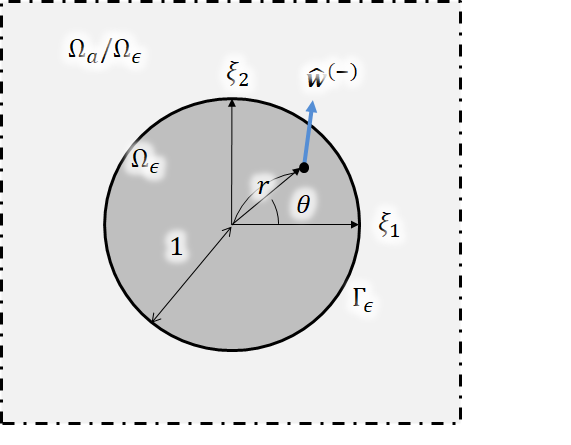
\includegraphics[height=5cm]{./figures/InHole.png}
		\caption{$\hat{\bm{w}}^{(-)}$ in $\Omega_{\epsilon}$}
		\label{fig:InHole}
	\end{center}
\end{figure}

式\eqref{eq:XiToRTh}のように$(\xi_{1},\xi_{2})$座標を$(r,\theta)$座標に変換する.
\begin{align}
	\xi_{1}=r\cos(\theta)
	\nonumber
	\\
	\xi_{2}=r\sin(\theta)
	\label{eq:XiToRTh}
\end{align}
$\Omega_\epsilon$内の$\hat{\bm{w}}^{(I-)}$に関するThe Airy stress function $\Phi^{(I-)}$は,
The Michell solution \eqref{eq:Michell}を用いて以下のように展開できる.
\begin{align}
	\Phi^{(I-)} =&A_{01}^{(I-)}r^2+A_{02}^{(I-)}r^2\ln(r)+A_{03}^{(I-)}\ln(r)+A_{04}^{(I-)}\theta
	\nonumber
	\\
	&+\Bigl(A_{11}^{(I-)}r^3+A_{12}^{(I-)}r\ln(r)+A_{14}^{(I-)}r^{-1}\Bigr)\cos(\theta)+A_{13}^{(I-)}r\theta \sin(\theta)
	\nonumber
	\\
	&+\Bigl(B_{11}^{(I-)}r^3+B_{12}^{(I-)}r\ln(r)+B_{14}^{(I-)}r^{-1}\Bigr)\sin(\theta)+B_{13}^{(I-)}r\theta \cos(\theta)
	\nonumber
	\\
	&+\sum_{m=2}^{\infty}\Bigl(A_{m1}^{(I-)}r^{m+2}+A_{m2}^{(I-)}r^{-m+2}
	+A_{m3}^{(I-)}r^{m}+A_{m4}^{(I-)}r^{-m}\Bigr)\cos(m\theta)
	\nonumber
	\\
	&+\sum_{m=2}^{\infty}\Bigl(B_{m1}^{(I-)}r^{m+2}+B_{m2}^{(I-)}r^{-m+2}
	+B_{m3}^{(I-)}r^{m}+B_{m4}^{(I-)}r^{-m}\Bigr)\sin(m\theta)
	\label{eq:AiryIn1}
\end{align}

$r\rightarrow0$において,$|\hat{\bm{w}}^{(I-)}|<\infty$,$|\hat{\sigma}^{(I-)}|<\infty$となる条件は以下のようになる,
\begin{align}
	A_{02}^{(I-)}=0,\hspace{1cm}A_{03}^{(I-)}=0,\hspace{1cm}A_{04}^{(I-)}=0&
	\nonumber
	\\
	A_{12}^{(I-)}=0,\hspace{1cm}A_{13}^{(I-)}=0,\hspace{1cm}A_{14}^{(I-)}=0&
	\nonumber
	\\
	B_{12}^{(I-)}=0,\hspace{1cm}B_{13}^{(I-)}=0,\hspace{1cm}B_{14}^{(I-)}=0&
	\nonumber
	\\
	A_{m2}^{(I-)}=0,\hspace{1cm}A_{m4}^{(I-)}=0&\hspace{1cm}(m\geq2)
	\nonumber
	\\
	B_{m2}^{(I-)}=0,\hspace{1cm}B_{m4}^{(I-)}=0&\hspace{1cm}(m\geq2)
	\label{eq:ConIn1}
\end{align}
ゆえに,式\eqref{eq:ConIn1}を用いて,$\hat{w}_{r}^{(I-)},\hat{w}_{\theta}^{(I-)},\hat{\sigma}_{rr}^{(I-)},\hat{\sigma}_{r\theta}^{(I-)}$を整理すると,以下のようになる.
\begin{align}
	2\mu^{b}\hat{w}_{r}^{(I-)} =&D_{1}^{(I-)}\cos(\theta)+D_{2}^{(I-)}\sin(\theta)
	\nonumber
	\\
	&+A_{01}^{(I-)}(\kappa^{b}-1)r
	\nonumber
	\\
	&+A_{11}^{(I-)}(\kappa^{b}-2)r^2\cos(\theta)
	+B_{11}^{(I-)}(\kappa^{b}-2)r^2\sin(\theta)
	\nonumber
	\\
	&+\sum_{m=2}^{\infty}\Bigl\{A_{m1}^{(I-)}(\kappa^{b}-m-1)r^{m+1}
	-A_{m3}^{(I-)}mr^{m-1}\Bigr\}\cos(m\theta)
	\nonumber
	\\
	&+\sum_{m=2}^{\infty}\Bigl\{B_{m1}^{(I-)}(\kappa^{b}-m-1)r^{m+1}
	-B_{m3}^{(I-)}mr^{m-1}\Bigr\}\sin(m\theta)
	\label{eq:URIn1}
\end{align}
\begin{align}
	2\mu^{b}\hat{w}_{\theta}^{(I-)} =&-D_{1}^{(I-)}\sin(\theta)+D_{2}^{(I-)}\cos(\theta)+D_{3}^{(I-)}r
	\nonumber
	\\
	&+A_{11}^{(I-)}(\kappa^{b}+2)r^2\sin(\theta)
	-B_{11}^{(I-)}(\kappa^{b}+2)r^2\cos(\theta)
	\nonumber
	\\
	&+\sum_{m=2}^{\infty}\Bigl\{A_{m1}^{(I-)}(\kappa^{b}+m+1)r^{m+1}
	+A_{m3}^{(I-)}mr^{m-1}\Bigr\}\sin(m\theta)
	\nonumber
	\\
	&+\sum_{m=2}^{\infty}\Bigl\{-B_{m1}^{(I-)}(\kappa^{b}+m+1)r^{m+1}
	-B_{m3}^{(I-)}mr^{m-1}\Bigr\}\cos(m\theta)
	\label{eq:UThIn1}
\end{align}
\begin{align}
	\hat{\sigma}_{rr}^{(I-)} =&2A_{01}^{(I-)}
	\nonumber
	\\
	&+2A_{11}^{(I-)}r\cos(\theta)
	+2B_{11}^{(I-)}r\sin(\theta)
	\nonumber
	\\
	&+\sum_{m=2}^{\infty}\Bigl\{-A_{m1}^{(I-)}(m+1)(m-2)r^{m}
	-A_{m3}^{(I-)}m(m-1)r^{m-2}\Bigr\}\cos(m\theta)
	\nonumber
	\\
	&+\sum_{m=2}^{\infty}\Bigl\{-B_{m1}^{(I-)}(m+1)(m-2)r^{m}
	-B_{m3}^{(I-)}m(m-1)r^{m-2}\Bigr\}\sin(m\theta)
	\label{eq:SigmaRRIn1}
\end{align}
\begin{align}
	\hat{\sigma}_{r\theta}^{(I-)} =
	&2A_{11}^{(I-)}r\sin(\theta)
	-2B_{11}^{(I-)}r\cos(\theta)
	\nonumber
	\\
	&+\sum_{m=2}^{\infty}\Bigl\{A_{m1}^{(I-)}m(m+1)r^{m}
	+A_{m3}^{(I-)}m(m-1)r^{m-2}\Bigr\}\sin(m\theta)
	\nonumber
	\\
	&+\sum_{m=2}^{\infty}\Bigl\{-B_{m1}^{(I-)}m(m+1)r^{m}
	-B_{m3}^{(I-)}m(m-1)r^{m-2}\Bigr\}\cos(m\theta)
	\label{eq:SigmaRThIn1}
\end{align}
\begin{align}
	\hat{\sigma}_{\theta\theta}^{(I-)} =&2A_{01}^{(I-)}
	\nonumber
	\\
	&+6A_{11}^{(I-)}r\cos(\theta)+6B_{11}^{(I-)}r\sin(\theta)
	\nonumber
	\\
	&+\sum_{m=2}^{\infty}\Bigl\{A_{m1}^{(I-)}(m+1)(m+2)r^{m}
	+A_{m3}^{(I-)}m(m-1)r^{m-2}\Bigr\}\cos(m\theta)
	\nonumber
	\\
	&+\sum_{m=2}^{\infty}\Bigl\{B_{m1}^{(I-)}(m+1)(m+2)r^{m}
	+B_{m3}^{(I-)}m(m-1)r^{m-2}\Bigr\}\sin(m\theta)
	\label{eq:SigmaThThIn1}
\end{align}
\newpage

\section{$\hat{\bm{w}}^{(I+)}$のThe Michell solutionによる表現}
\begin{figure}[ht]
	\begin{center}
		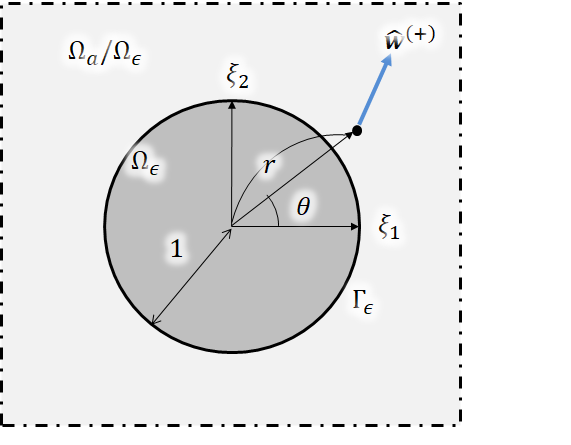
\includegraphics[height=5cm]{./figures/OutHole.png}
		\caption{$\hat{\bm{w}}^{(+)}$ outside $\Omega_{\epsilon}$}
		\label{fig:OutHole}
	\end{center}
\end{figure}

一方,$\Omega_{a}\backslash\Omega_\epsilon$におけるThe Airy stress function $\Phi^{(I+)}$に関しても同様に,
The Michell solution \eqref{eq:Michell}を用いて以下のように展開できる.
\begin{align}
\Phi^{(I+)} =&A_{01}^{(I+)}r^2+A_{02}^{(I+)}r^2\ln(r)+A_{03}^{(I+)}\ln(r)+A_{04}^{(I+)}\theta
\nonumber
\\
&+\Bigl(A_{11}^{(I+)}r^3+A_{12}^{(I+)}r\ln(r)+A_{14}^{(I+)}r^{-1}\Bigr)\cos(\theta)+A_{13}^{(I+)}r\theta \sin(\theta)
\nonumber
\\
&+\Bigl(B_{11}^{(I+)}r^3+B_{12}^{(I+)}r\ln(r)+B_{14}^{(I+)}r^{-1}\Bigr)\sin(\theta)+B_{13}^{(I+)}r\theta \cos(\theta)
\nonumber
\\
&+\sum_{m=2}^{\infty}\Bigl(A_{m1}^{(I+)}r^{m+2}+A_{m2}^{(I+)}r^{-m+2}
+A_{m3}^{(I+)}r^{m}+A_{m4}^{(I+)}r^{-m}\Bigr)\cos(m\theta)
\nonumber
\\
&+\sum_{m=2}^{\infty}\Bigl(B_{m1}^{(I+)}r^{m+2}+B_{m2}^{(I+)}r^{-m+2}
+B_{m3}^{(I+)}r^{m}+B_{m4}^{(I+)}r^{-m}\Bigr)\sin(m\theta)
\label{eq:AiryOut1}
\end{align}

$r\rightarrow\infty$において,$|\hat{\bm{w}}^{(I+)}|\rightarrow0$となる条件は以下のようになる,
\begin{align}
D_{1}^{(I+)}=0,\hspace{1cm}
D_{2}^{(I+)}=0,\hspace{1cm}
D_{3}^{(I+)}=0&
\nonumber
\\
A_{01}^{(I+)}=0,\hspace{1cm}A_{02}^{(I+)}=0&
\nonumber
\\
A_{11}^{(I+)}=0,\hspace{1cm}A_{12}^{(I+)}=0,\hspace{1cm}A_{13}^{(I+)}=0&
\nonumber
\\
B_{11}^{(I+)}=0,\hspace{1cm}B_{12}^{(I+)}=0,\hspace{1cm}B_{13}^{(I+)}=0&
\nonumber
\\
A_{m1}^{(I+)}=0,\hspace{1cm}A_{m3}^{(I+)}=0&\hspace{1cm}(m\geq2)
\nonumber
\\
B_{m1}^{(I+)}=0,\hspace{1cm}B_{m3}^{(I+)}=0&\hspace{1cm}(m\geq2)
\label{eq:ConOut1}
\end{align}
ゆえに,式\eqref{eq:ConOut1}を用いて$\hat{w}_{r}^{(I+)},\hat{w}_{\theta}^{(I+)},\hat{\sigma}_{rr}^{(I+)},\hat{\sigma}_{r\theta}^{(I+)}$を整理すると,以下のようになる.
\begin{align}
	2\mu^{a}\hat{w}_{r}^{(I+)} =&-A_{03}^{(I+)}r^{-1}
	\nonumber
	\\
	&+A_{14}^{(I+)}r^{-2}\cos(\theta)
	+B_{14}^{(I+)}r^{-2}\sin(\theta)
	\nonumber
	\\
	&+\sum_{m=2}^{\infty}\Bigl\{A_{m2}^{(I+)}(\kappa^{a}+m-1)r^{-m+1}
	+A_{m4}^{(I+)}mr^{-m-1}\Bigr\}\cos(m\theta)
	\nonumber
	\\
	&+\sum_{m=2}^{\infty}\Bigl\{B_{m2}^{(I+)}(\kappa^{a}+m-1)r^{-m+1}
	+B_{m4}^{(I+)}mr^{-m-1}\Bigr\}\sin(m\theta)
	\label{eq:UROut1}
\end{align}
\begin{align}
	2\mu^{a}\hat{w}_{\theta}^{(I+)} =&-A_{04}^{(I+)}r^{-1}
	\nonumber
	\\
	&+A_{14}^{(I+)}r^{-2}\sin(\theta)
	-B_{14}^{(I+)}r^{-2}\cos(\theta)
	\nonumber
	\\
	&+\sum_{m=2}^{\infty}\Bigl\{-A_{m2}^{(I+)}(\kappa^{a}-m+1)r^{-m+1}
	+A_{m4}^{(I+)}mr^{-m-1}\Bigr\}\sin(m\theta)
	\nonumber
	\\
	&+\sum_{m=2}^{\infty}\Bigl\{B_{m2}^{(I+)}(\kappa^{a}-m+1)r^{-m+1}
	-B_{m4}^{(I+)}mr^{-m-1}\Bigr\}\cos(m\theta)
	\label{eq:UThOut1}
\end{align}
\begin{align}
	\hat{\sigma}_{rr}^{(I+)} =&A_{03}^{(I+)}r^{-2}
	\nonumber
	\\
	&-2A_{14}^{(I+)}r^{-3}\cos(\theta)
	-2B_{14}^{(I+)}r^{-3}\sin(\theta)
	\nonumber
	\\
	&+\sum_{m=2}^{\infty}\Bigl\{
	-A_{m2}^{(I+)}(m+2)(m-1)r^{-m}
	-A_{m4}^{(I+)}m(m+1)r^{-m-2}\Bigr\}\cos(m\theta)
	\nonumber
	\\
	&+\sum_{m=2}^{\infty}\Bigl\{
	-B_{m2}^{(I+)}(m+2)(m-1)r^{-m}
	-B_{m4}^{(I+)}m(m+1)r^{-m-2}\Bigr\}\sin(m\theta)
	\label{eq:SigmaRROut1}
\end{align}
\begin{align}
	\hat{\sigma}_{r\theta}^{(I+)} =&A_{04}^{(I+)}r^{-2}
	\nonumber
	\\
	&-2A_{14}^{(I+)}r^{-3}\sin(\theta)
	+2B_{14}^{(I+)}r^{-3}\cos(\theta)
	\nonumber
	\\
	&+\sum_{m=2}^{\infty}\Bigl\{
	-A_{m2}^{(I+)}m(m-1)r^{-m}
	-A_{m4}^{(I+)}m(m+1)r^{-m-2}\Bigr\}\sin(m\theta)
	\nonumber
	\\
	&+\sum_{m=2}^{\infty}\Bigl\{
	B_{m2}^{(I+)}m(m-1)r^{-m}
	+B_{m4}^{(I+)}m(m+1)r^{-m-2}\Bigr\}\cos(m\theta)
	\label{eq:SigmaRThOut1}
\end{align}
\begin{align}
	\hat{\sigma}_{\theta\theta}^{(I+)} =&-A_{03}^{(I+)}r^{-2}
	\nonumber
	\\
	&2A_{14}^{(I+)}r^{-3}\cos(\theta)+2B_{14}^{(I+)}r^{-3}\sin(\theta)
	\nonumber
	\\
	&+\sum_{m=2}^{\infty}\Bigl\{A_{m2}^{(I+)}(m-1)(m-2)r^{-m}
	+A_{m4}^{(I+)}m(m+1)r^{-m-2}\Bigr\}\cos(m\theta)
	\nonumber
	\\
	&+\sum_{m=2}^{\infty}\Bigl\{B_{m2}^{(I+)}(m-1)(m-2)r^{-m}
	+B_{m4}^{(I+)}m(m+1)r^{-m-2}\Bigr\}\sin(m\theta)
	\label{eq:SigmaThThOut1}
\end{align}
\newpage

\section{$\Gamma_{\epsilon}$上の境界条件から得られる等式}
$D_{i}^{*(I-)},A_{ij}^{*(I-)},B_{ij}^{*(I-)},A_{ij}^{*(I+)},B_{ij}^{*(I+)}$を次式のように定義する.
\begin{align}
	D_{i}^{(I-)}=2\mu^{b}D_{i}^{*(I-)},\hspace{1cm}A_{ij}^{(I-)}=2\mu^{b}A_{ij}^{*(I-)},\hspace{1cm}
	B_{ij}^{(I-)}=2\mu^{b}B_{ij}^{*(I-)}&
	\nonumber
	\\
	A_{ij}^{(I+)}=2\mu^{a}A_{ij}^{*(I+)},\hspace{1cm}
	B_{ij}^{(I+)}=2\mu^{a}B_{ij}^{*(I+)}&
	\label{eq:ChangeCoef}
\end{align}

$\Gamma_{\epsilon}(r=1)$上の変位および応力ベクトルの境界条件\eqref{eq:GovDisturUBC1}\eqref{eq:GovDisturSBC1}より,次の4つの等式が得られる.
\begin{align}
	\hat{w}_{r}^{(I-)}-\hat{w}_{r}^{(I+)} =&A_{01}^{*(I-)}(\kappa^{b}-1)-\Bigl(-A_{03}^{*(I+)}\Bigr)
	\nonumber
	\\
	&+\Bigl\{D_{1}^{*(I-)}+A_{11}^{*(I-)}(\kappa^{b}-2)
	-\Bigl(A_{14}^{*(I+)}\Bigr)\Bigr\}\cos(\theta)
	\nonumber
	\\
	&+\Bigl\{D_{2}^{*(I-)}+B_{11}^{*(I-)}(\kappa^{b}-2)
	-\Bigl(B_{14}^{*(I+)}\Bigr)\Bigr\}\sin(\theta)
	\nonumber
	\\
	&+\sum_{m=2}^{\infty}\Bigl\{A_{m1}^{*(I-)}(\kappa^{b}-m-1)
	-A_{m3}^{*(I-)}m
	\nonumber
	\\
	&\hspace{1.0cm}-\Bigl(A_{m2}^{*(I+)}(\kappa^{a}+m-1)
	+A_{m4}^{*(I+)}m\Bigr)\Bigr\}\cos(m\theta)
	\nonumber
	\\
	&+\sum_{m=2}^{\infty}\Bigl\{B_{m1}^{*(I-)}(\kappa^{b}-m-1)
	-B_{m3}^{*(I-)}m
	\nonumber
	\\
	&\hspace{1.0cm}-\Bigl(B_{m2}^{*(I+)}(\kappa^{a}+m-1)
	+B_{m4}^{*(I+)}m\Bigr)\Bigr\}\sin(m\theta)
	\nonumber
	\\
	=&u_{r}(\bm{z})
	\nonumber
	\\
	=&u_{x_{1}}(\bm{z})\cos(\theta)+u_{x_{2}}(\bm{z})\sin(\theta)
	\label{eq:UR1eq}
\end{align}
\begin{align}
	\hat{w}_{\theta}^{(I-)}-\hat{w}_{\theta}^{(I+)} =&D_{3}^{*(I-)}-\Bigl(-A_{04}^{*(I+)}\Bigr)
	\nonumber
	\\
	&+\Bigl\{-D_{1}^{*(I-)}+A_{11}^{*(I-)}(\kappa^{b}+2)
	-\Bigl(A_{14}^{*(I+)}\Bigr)\Bigr\}\sin(\theta)
	\nonumber
	\\
	&+\Bigl\{D_{2}^{*(I-)}-B_{11}^{*(I-)}(\kappa^{b}+2)
	-\Bigl(-B_{14}^{*(I+)}\Bigr)\Bigr\}\cos(\theta)
	\nonumber
	\\
	&+\sum_{m=2}^{\infty}\Bigl\{A_{m1}^{*(I-)}(\kappa^{b}+m+1)
	+A_{m3}^{*(I-)}m
	\nonumber
	\\
	&\hspace{1.0cm}-\Bigl(-A_{m2}^{*(I+)}(\kappa^{a}-m+1)
	+A_{m4}^{*(I+)}m\Bigr)\Bigr\}\sin(m\theta)
	\nonumber
	\\
	&+\sum_{m=2}^{\infty}\Bigl\{-B_{m1}^{*(I-)}(\kappa^{b}+m+1)
	-B_{m3}^{*(I-)}m
	\nonumber
	\\
	&\hspace{1.0cm}-\Bigl(B_{m2}^{*(I+)}(\kappa^{a}-m+1)
	-B_{m4}^{*(I+)}m\Bigr)\Bigr\}\cos(m\theta)
	\nonumber
	\\
	=&u_{\theta}(\bm{z})
	\nonumber
	\\
	=&-u_{x_{1}}(\bm{z})\sin(\theta)+u_{x_{2}}(\bm{z})\cos(\theta)
	\label{eq:UTh1eq}
\end{align}
\begin{align}
	\hat{\sigma}_{rr}^{(I-)}-\hat{\sigma}_{rr}^{(I+)} =
	&2A_{01}^{(I-)}-\Bigl(A_{03}^{(I+)}\Bigr)
	\nonumber
	\\
	&+\Bigl\{2A_{11}^{(I-)}
	-\Bigl(-2A_{14}^{(I+)}\Bigr)\Bigr\}\cos(\theta)
	\nonumber
	\\
	&+\Bigl\{2B_{11}^{(I-)}
	-\Bigl(-2B_{14}^{(I+)}\Bigr)\Bigr\}\sin(\theta)
	\nonumber
	\\
	&+\sum_{m=2}^{\infty}\Bigl\{
	-A_{m1}^{(I-)}(m+1)(m-2)-A_{m3}^{(I-)}m(m-1)
	\nonumber
	\\
	&\hspace{1.0cm}-\Bigl(-A_{m2}^{(I+)}(m+2)(m-1)-A_{m4}^{(I+)}m(m+1)\Bigr)
	\Bigr\}\cos(m\theta)
	\nonumber
	\\
	&+\sum_{m=2}^{\infty}\Bigl\{
	-B_{m1}^{(I-)}(m+1)(m-2)-B_{m3}^{(I-)}m(m-1)
	\nonumber
	\\
	&\hspace{1.0cm}-\Bigl(-B_{m2}^{(I+)}(m+2)(m-1)-B_{m4}^{(I+)}m(m+1)\Bigr)
	\Bigr\}\sin(m\theta)
	\nonumber
	\\
	=&0
	\label{eq:SigmaRReq}
\end{align}
\begin{align}
	\hat{\sigma}_{r\theta}^{(I-)}-\hat{\sigma}_{r\theta}^{(I+)} =
	&-A_{04}^{(I+)}
	\nonumber
	\\
	&+\Bigl\{2A_{11}^{(I-)}
	-\Bigl(-2A_{14}^{(I+)}\Bigr)\Bigr\}\sin(\theta)
	\nonumber
	\\
	&+\Bigl\{-2B_{11}^{(I-)}
	-\Bigl(2B_{14}^{(I+)}\Bigr)\Bigr\}\cos(\theta)
	\nonumber
	\\
	&+\sum_{m=2}^{\infty}\Bigl\{
 	A_{m1}^{(I-)}m(m+1)+A_{m3}^{(I-)}m(m-1)
	\nonumber
	\\
	&\hspace{1.0cm}-\Bigl(-A_{m2}^{(I+)}m(m-1)-A_{m4}^{(I+)}m(m+1)\Bigr)
	\Bigr\}\sin(m\theta)
	\nonumber
	\\
	&+\sum_{m=2}^{\infty}\Bigl\{
	-B_{m1}^{(I-)}m(m+1)-B_{m3}^{(I-)}m(m-1)
	\nonumber
	\\
	&\hspace{1.0cm}-\Bigl(B_{m2}^{(I+)}m(m-1)+B_{m4}^{(I+)}m(m+1)\Bigr)
	\Bigr\}\cos(m\theta)
	\nonumber
	\\
	=&0
	\label{eq:SigmaRTh1eq}
\end{align}
\newpage

\section{The Michell solutionの係数に関する連立方程式}
任意の$0\leq\pi\leq2\pi$に対して\eqref{eq:UR1eq}~\eqref{eq:SigmaRTh1eq}が成立するためには
$1$,$\cos(m\theta)$,$\sin(m\theta)$$(m\geq1)$の係数が0である必要がある.ゆえに,次下の連立方程式が得られる.

1の係数:
\begin{align}
	\left(
	\begin{array}{cccc}
		{\dsp\frac{1}{2\mu^b}}& 0 & 0 & {\dsp\frac{1}{2\mu^a}} \\
		0 & {\dsp\frac{\kappa^b-1}{2\mu^b}} & {\dsp\frac{1}{2\mu^a}} & 0 \\
		0 & 4 & -2 & 0 \\
		0 & 0 & 0 & -2 \\
	\end{array}
	\right)
	\left(
	\begin{array}{c}
		D_{3}^{(I-)} \\
	 	A_{01}^{(I-)} \\
		A_{03}^{(I+)}\\
	 	A_{04}^{(I+)} \\
	\end{array}
	\right)
	=
	\left(
	\begin{array}{c}
		0 \\
	 	0 \\
		0 \\
	 	0 \\
	\end{array}
	\right)
\end{align}
$\cos(\theta),\sin(\theta)$の係数:
\begin{align}
	\left(
	\begin{array}{ccc}
		{\dsp\frac{1}{2\mu^b}}& {\dsp\frac{\kappa^b-2}{2\mu^b}} & {\dsp-\frac{1}{2\mu^a}} \\
		{\dsp-\frac{1}{2\mu^b}} & {\dsp\frac{\kappa^b+2}{2\mu^b}} & {\dsp-\frac{1}{2\mu^a}} \\
		0 & 4 & 4 \\
	\end{array}
	\right)
	\left(
	\begin{array}{c}
		D_{1}^{(I-)} \\
	 	A_{11}^{(I-)} \\
	 	A_{14}^{(I+)} \\
	\end{array}
	\right)
	=
	\left(
	\begin{array}{c}
		u_{x_{1}}(\bm{z}) \\
	 	-u_{x_{1}}(\bm{z}) \\
	 	0 \\
	\end{array}
	\right)
\end{align}
\begin{align}
	\left(
	\begin{array}{ccc}
		{\dsp\frac{1}{2\mu^b}}& {\dsp\frac{\kappa^b-2}{2\mu^b}} & {\dsp-\frac{1}{2\mu^a}} \\
		{\dsp\frac{1}{2\mu^b}} & {\dsp-\frac{\kappa^b+2}{2\mu^b}} & {\dsp\frac{1}{2\mu^a}} \\
		0 & -4 & -4 \\
	\end{array}
	\right)
	\left(
	\begin{array}{c}
		D_{2}^{(I-)} \\
	 	B_{11}^{(I-)} \\
	 	B_{14}^{(I+)} \\
	\end{array}
	\right)
	=
	\left(
	\begin{array}{c}
		u_{x_{2}}(\bm{z}) \\
	 	u_{x_{2}}(\bm{z}) \\
	 	0 \\
	\end{array}
	\right)
\end{align}
\newpage
$\cos(m\theta),\sin(m\theta)$の係数$(m\geq2)$:
\begin{align}
	\left(
	\begin{array}{cccc}
		{\dsp\frac{ \kappa^b-m-1}{2\mu^{b}}}& {\dsp-\frac{m}{2\mu^{b}}} &
		{\dsp-\frac{\kappa^a+m-1}{2\mu^{a}}} & {\dsp-\frac{m}{2\mu^{a}}} \\
		{\dsp\frac{\kappa^b+m+1}{2\mu^{b}}} & {\dsp\frac{m}{2\mu^{b}}} &
		{\dsp\frac{\kappa^a-m+1}{2\mu^{a}}} & {\dsp-\frac{m}{2\mu^{a}}} \\
		-(m+1)(m-2) & -m(m-1) & (m+2)(m-1) & m(m+1) \\
		m(m+1) & m(m-1) & m(m-1) & m(m+1)\\
	\end{array}
	\right)
	\left(
	\begin{array}{c}
		A_{m1}^{(I-)} \\
	 	A_{m3}^{(I-)} \\
		A_{m2}^{(I+)}\\
	 	A_{m4}^{(I+)} \\
	\end{array}
	\right)
	=
	\left(
	\begin{array}{c}
		0 \\
	 	0 \\
		0 \\
	 	0 \\
	\end{array}
	\right)
\end{align}
\begin{align}
	\left(
	\begin{array}{cccc}
		{\dsp\frac{ \kappa^b-m-1}{2\mu^{b}}}& {\dsp-\frac{m}{2\mu^{b}}} &
		{\dsp-\frac{\kappa^a+m-1}{2\mu^{a}}} & {\dsp-\frac{m}{2\mu^{a}}} \\
		{\dsp-\frac{\kappa^b+m+1}{2\mu^{b}}} & {\dsp-\frac{m}{2\mu^{b}}} &
		{\dsp-\frac{\kappa^a-m+1}{2\mu^{a}}} & {\dsp \frac{m}{2\mu^{a}}} \\
		-(m+1)(m-2) & -m(m-1) & (m+2)(m-1) & m(m+1) \\
		-m(m+1) & -m(m-1) & -m(m-1) & -m(m+1)\\
	\end{array}
	\right)
	\left(
	\begin{array}{c}
		B_{m1}^{(I-)} \\
	 	B_{m3}^{(I-)} \\
		B_{m2}^{(I+)}\\
	 	B_{m4}^{(I+)} \\
	\end{array}
	\right)
	=
	\left(
	\begin{array}{c}
		0 \\
	 	0 \\
		0 \\
	 	0 \\
	\end{array}
	\right)
\end{align}
これらの連立方程式を解くと,
\begin{align}
	D_{1}^{(I-)}=2\mu^{b}u_{x_{1}}(\bm{z}),\hspace{0.5cm}
	D_{2}^{(I-)}=2\mu^{b}u_{x_{2}}(\bm{z}),\hspace{0.5cm}D_{3}^{(I-)}=0
	\nonumber
	\\
	A_{ij}^{(I\pm)}=0,\hspace{0.5cm}
	B_{ij}^{(I\pm)}=0,\hspace{0.5cm}(i\geq0,1\leq j\leq4)
\end{align}
以上から,$\hat{\bm{w}}^{(I)}$は以下のように求まる.
\begin{align}
	\hat{w}_{r}^{(I-)}=u_{x_{1}}(\bm{z})\cos(\theta)+u_{x_{2}}(\bm{z})\sin(\theta)
	\nonumber
	\\
	\hat{w}_{\theta}^{(I-)}=-u_{x_{1}}(\bm{z})\sin(\theta)+u_{x_{2}}(\bm{z})\cos(\theta)
	\label{eq:w1InSol}
	\\
	\hat{w}_{r}^{(I+)}=0,\hspace{1.0cm}\hat{w}_{\theta}^{(I+)}=0\hspace{1.0cm}
	\label{eq:w1OutSol}
\end{align}

\newpage


\section{$\hat{\bm{w}}^{(I\hspace{-.15em}I-)}$,$\hat{\bm{w}}^{(I\hspace{-.15em}I+)}$の導出}
境界$\Gamma_{\epsilon}$上の極座標$(1,\theta)$における$\xi_1,\xi_2$座標は$(\xi_1,\xi_2)=(\cos(\theta),\sin(\theta))$,
法線ベクトルの$\xi_1,\xi_2$成分は$(n_{\xi_1},n_{\xi_2})=(\cos(\theta),\sin(\theta))$である.
ゆえに$\Gamma_\epsilon$上の境界条件\eqref{eq:GovDisturUBC2}における変位$\bm{u}^{(I\hspace{-.15em}I)}$の$\xi_1,\xi_2$成分は次式で表される.
\begin{align}
	u_{\xi_1}^{(I\hspace{-.15em}I)}=&\xi_{j} u_{x_{1},j}(\bm{z})
	\nonumber
	\\
	=&u_{x_{1},x_{1}}(\bm{z})\cos(\theta)+u_{x_{1},x_{2}}(\bm{z})\sin(\theta)
	\\
	u_{\xi_2}^{(I\hspace{-.15em}I)}=
	&u_{x_{2},x_{1}}(\bm{z})\cos(\theta)+u_{x_{2},x_{2}}(\bm{z})\sin(\theta)
\end{align}
ゆえに,$\bm{u}^{(I\hspace{-.15em}I)}$の$r,\theta$方向成分は以下のようになる.
\begin{align}
	u_{r}^{(I\hspace{-.15em}I)}=
		&u_{\xi_1}^{(I\hspace{-.15em}I)}\cos(\theta)+u_{\xi_2}^{(I\hspace{-.15em}I)}\sin(\theta)
		\nonumber
		\\
		=&u_{x_{1},x_{1}}(\bm{z})\cos^2(\theta)+\bigl\{u_{x_{1},x_{2}}(\bm{z})
		+u_{x_{2},x_{1}}(\bm{z})\bigr\}\sin(\theta)\cos(\theta)
		+u_{x_{2},x_{2}}(\bm{z})\sin^2(\theta)
		\nonumber
		\\
		=&\frac{1}{2}\bigl\{u_{x_{1},x_{1}}(\bm{z})+u_{x_{2},x_{2}}(\bm{z})\bigr\}
		+\frac{1}{2}\bigl\{u_{x_{1},x_{1}}(\bm{z})-u_{x_{2},x_{2}}(\bm{z})\bigr\}\cos(2\theta)
		\nonumber
		\\
		&\quad+\frac{1}{2}\bigl\{u_{x_{1},x_{2}}(\bm{z})+u_{x_{2},x_{1}}(\bm{z})\bigr\}\sin(2\theta)
		\\
	u_{\theta}^{(I\hspace{-.15em}I)}=
		&-u_{\xi_1}^{(I\hspace{-.15em}I)}\sin(\theta)+u_{\xi_2}^{(I\hspace{-.15em}I)}\cos(\theta)
		\nonumber
		\\
		=&-\bigl\{u_{x_{1},x_{1}}(\bm{z})-u_{x_{2},x_{2}}(\bm{z})\bigr\}\cos(\theta)\sin(\theta)
		-u_{x_{1},x_{2}}(\bm{z})\sin^2(\theta)+u_{x_{2},x_{1}}(\bm{z})\cos^2(\theta)
		\nonumber
		\\
		=&-\frac{1}{2}\bigl\{u_{x_{1},x_{2}}(\bm{z})-u_{x_{2},x_{1}}(\bm{z})\bigr\}
		+\frac{1}{2}\bigl\{u_{x_{1},x_{2}}(\bm{z})+u_{x_{2},x_{1}}(\bm{z})\bigr\}\cos(2\theta)
		\nonumber
		\\
		&\quad-\frac{1}{2}\bigl\{u_{x_{1},x_{1}}(\bm{z})-u_{x_{2},x_{2}}(\bm{z})\bigr\}\sin(2\theta)
\end{align}

また,$\Gamma_\epsilon$上の境界条件\eqref{eq:GovDisturSBC2}における応力ベクトル$\bm{t}^{(I\hspace{-.15em}I)}$の$\xi_1,\xi_2$成分は次式になる.
\begin{align}
	t_{\xi_1}^{(I\hspace{-.15em}I)}=&C_{1jkl}^{a}u_{k,l}^{}(\bm{z})n_{j}
		\nonumber
		\\
		=&\mu^a\Bigl\{\frac{\kappa^a+1}{\kappa^a-1} u_{x_{1},x_{1}}(\bm{z})
		+\frac{3-\kappa^a}{\kappa^a-1} u_{x_{2},x_{2}}(\bm{z})\Bigr\}\cos(\theta)
		\nonumber
		\\
		&\quad+\mu^a\bigl\{u_{x_{1},x_{2}}(\bm{z})+u_{x_{2},x_{1}}(\bm{z})\bigr\}\sin(\theta)
	\\
	t_{\xi_2}^{(I\hspace{-.15em}I)}=&C_{2jkl}^{a}u_{k,l}^{}(\bm{z})n_{j}
		\nonumber
		\\
		=&\mu^a \bigl\{u_{x_{1},x_{2}}(\bm{z})+u_{x_{2},x_{1}}(\bm{z})\bigr\}\cos(\theta)
		\nonumber
		\\
		&\quad+\mu^a\Bigl\{ \frac{3-\kappa^a}{\kappa^a-1} u_{x_{1},x_{1}}(\bm{z})
		+\frac{\kappa^a+1}{\kappa^a-1} u_{x_{2},x_{2}}(\bm{z})\Bigr\}\sin(\theta)
\end{align}
ゆえに,$\bm{t}^{(I\hspace{-.15em}I)}$の$r,\theta$方向成分は以下のようになる.
\begin{align}
	t_{r}^{(I\hspace{-.15em}I)}
		=&t_{\xi_1}^{(I\hspace{-.15em}I)}\cos(\theta)+t_{\xi_2}^{(I\hspace{-.15em}I)}\sin(\theta)
			\nonumber
			\\
		=&\mu^a\Bigl\{\frac{\kappa^a+1}{\kappa^a-1} u_{x_{1},x_{1}}(\bm{z})
			+\frac{3-\kappa^a}{\kappa^a-1} u_{x_{2},x_{2}}(\bm{z})\Bigr\}\cos^2(\theta)
			\nonumber
			\\
			&\quad+2\mu^a\bigl\{u_{x_{1},x_{2}}(\bm{z})
			+u_{x_{2},x_{1}}(\bm{z})\bigr\}\sin(\theta)\cos(\theta)
			\nonumber
			\\
			&\quad+\mu^a\Bigl\{ \frac{3-\kappa^a}{\kappa^a-1} u_{x_{1},x_{1}}(\bm{z})
			+\frac{\kappa^a+1}{\kappa^a-1} u_{x_{2},x_{2}}(\bm{z})\Bigr\}\sin^2(\theta)
			\nonumber
			\\
		=&\frac{2\mu^a}{\kappa^a-1}\Bigl\{ u_{x_{1},x_{1}}(\bm{z})
			+ u_{x_{2},x_{2}}(\bm{z})\Bigr\}
			\nonumber
			\\
			&\quad+\mu^a\bigl\{u_{x_{1},x_{2}}(\bm{z})
			+u_{x_{2},x_{1}}(\bm{z})\bigr\}\sin(2\theta)
			\nonumber
			\\
			&\quad+\mu^a\Bigl\{ u_{x_{1},x_{1}}(\bm{z})
			+ u_{x_{2},x_{2}}(\bm{z})\Bigr\}\cos(2\theta)
			\\
	t_{\theta}^{(I\hspace{-.15em}I)}				
		=&-t_{\xi_1}^{(I\hspace{-.15em}I)}\sin(\theta)+t_{\xi_2}^{(I\hspace{-.15em}I)}\cos(\theta)
			\nonumber
			\\
		=&-2\mu^a \bigl\{u_{x_{1},x_{2}}(\bm{z})-u_{x_{2},x_{1}}(\bm{z})\bigr\}\cos(\theta)\sin(\theta)
			\nonumber
			\\
			&+\mu^a \bigl\{u_{x_{1},x_{2}}(\bm{z})+u_{x_{2},x_{1}}(\bm{z})\bigr\}
			\bigl(\cos^2(\theta)-\sin^2(\theta)\bigr)
			\nonumber
			\\
		=&-\mu^a \bigl\{u_{x_{1},x_{2}}(\bm{z})-u_{x_{2},x_{1}}(\bm{z})\bigr\}\sin(2\theta)
			\nonumber
			\\
			&+\mu^a \bigl\{u_{x_{1},x_{2}}(\bm{z})+u_{x_{2},x_{1}}(\bm{z})\bigr\}\cos(2\theta)
\end{align}

$\Gamma_{\epsilon}$上の変位および応力の境界条件\eqref{eq:GovDisturUBC2}\eqref{eq:GovDisturSBC2}より次の4つの等式が得られる.

\begin{align}
	\hat{w}_{r}^{(I\hspace{-.15em}I-)}-\hat{w}_{r}^{(I\hspace{-.15em}I+)} =
	&A_{01}^{*(I\hspace{-.15em}I-)}(\kappa^{b}-1)-\Bigl(-A_{03}^{*(I\hspace{-.15em}I+)}\Bigr)
	\nonumber
	\\
	&+\Bigl\{D_{1}^{*(I\hspace{-.15em}I-)}+A_{11}^{*(I\hspace{-.15em}I-)}(\kappa^{b}-2)
	-\Bigl(A_{14}^{*(I\hspace{-.15em}I+)}\Bigr)\Bigr\}\cos(\theta)
	\nonumber
	\\
	&+\Bigl\{D_{2}^{*(I\hspace{-.15em}I-)}+B_{11}^{*(I\hspace{-.15em}I-)}(\kappa^{b}-2)
	-\Bigl(B_{14}^{*(I\hspace{-.15em}I+)}\Bigr)\Bigr\}\sin(\theta)
	\nonumber
	\\
	&+\sum_{m=2}^{\infty}\Bigl\{A_{m1}^{*(I\hspace{-.15em}I-)}(\kappa^{b}-m-1)
	-A_{m3}^{*(I\hspace{-.15em}I-)}m
	\nonumber
	\\
	&\hspace{1.0cm}-\Bigl(A_{m2}^{*(I\hspace{-.15em}I+)}(\kappa^{a}+m-1)
	+A_{m4}^{*(I\hspace{-.15em}I+)}m\Bigr)\Bigr\}\cos(m\theta)
	\nonumber
	\\
	&+\sum_{m=2}^{\infty}\Bigl\{B_{m1}^{*(I\hspace{-.15em}I-)}(\kappa^{b}-m-1)
	-B_{m3}^{*(I\hspace{-.15em}I-)}m
	\nonumber
	\\
	&\hspace{1.0cm}-\Bigl(B_{m2}^{*(I\hspace{-.15em}I+)}(\kappa^{a}+m-1)
	+B_{m4}^{*(I\hspace{-.15em}I+)}m\Bigr)\Bigr\}\sin(m\theta)
	\nonumber
	\\
	=&u_{r}^{(I\hspace{-.15em}I)}
	\nonumber
	\\
	=&\frac{1}{2}\bigl\{u_{x_{1},x_{1}}(\bm{z})+u_{x_{2},x_{2}}(\bm{z})\bigr\}
	+\frac{1}{2}\bigl\{u_{x_{1},x_{1}}(\bm{z})-u_{x_{2},x_{2}}(\bm{z})\bigr\}\cos(2\theta)
	\nonumber
	\\
	&+\frac{1}{2}\bigl\{u_{x_{1},x_{2}}(\bm{z})+u_{x_{2},x_{1}}(\bm{z})\bigr\}\sin(2\theta)
	\label{eq:UR2eq}
\end{align}

\begin{align}
	\hat{w}_{\theta}^{(I\hspace{-.15em}I-)}-\hat{w}_{\theta}^{(I\hspace{-.15em}I+)} =&D_{3}^{*(I\hspace{-.15em}I-)}-\Bigl(-A_{04}^{*(I\hspace{-.15em}I+)}\Bigr)
	\nonumber
	\\
	&+\Bigl\{-D_{1}^{*(I\hspace{-.15em}I-)}+A_{11}^{*(I\hspace{-.15em}I-)}(\kappa^{b}+2)
	-\Bigl(A_{14}^{*(I\hspace{-.15em}I+)}\Bigr)\Bigr\}\sin(\theta)
	\nonumber
	\\
	&+\Bigl\{D_{2}^{*(I\hspace{-.15em}I-)}-B_{11}^{*(I\hspace{-.15em}I-)}(\kappa^{b}+2)
	-\Bigl(-B_{14}^{*(I\hspace{-.15em}I+)}\Bigr)\Bigr\}\cos(\theta)
	\nonumber
	\\
	&+\sum_{m=2}^{\infty}\Bigl\{A_{m1}^{*(I\hspace{-.15em}I-)}(\kappa^{b}+m+1)
	+A_{m3}^{*(I\hspace{-.15em}I-)}m
	\nonumber
	\\
	&\hspace{1.0cm}-\Bigl(-A_{m2}^{*(I\hspace{-.15em}I+)}(\kappa^{a}-m+1)
	+A_{m4}^{*(I\hspace{-.15em}I+)}m\Bigr)\Bigr\}\sin(m\theta)
	\nonumber
	\\
	&+\sum_{m=2}^{\infty}\Bigl\{-B_{m1}^{*(I\hspace{-.15em}I-)}(\kappa^{b}+m+1)
	-B_{m3}^{*(I\hspace{-.15em}I-)}m
	\nonumber
	\\
	&\hspace{1.0cm}-\Bigl(B_{m2}^{*(I\hspace{-.15em}I+)}(\kappa^{a}-m+1)
	-B_{m4}^{*(I\hspace{-.15em}I+)}m\Bigr)\Bigr\}\cos(m\theta)
	\nonumber
	\\
	=&u_{\theta}^{(I\hspace{-.15em}I)}
	\nonumber
	\\
	=&-\frac{1}{2}\bigl\{u_{x_{1},x_{2}}(\bm{z})-u_{x_{2},x_{1}}(\bm{z})\bigr\}
	+\frac{1}{2}\bigl\{u_{x_{1},x_{2}}(\bm{z})+u_{x_{2},x_{1}}(\bm{z})\bigr\}\cos(2\theta)
	\nonumber
	\\
	&-\frac{1}{2}\bigl\{u_{x_{1},x_{1}}(\bm{z})-u_{x_{2},x_{2}}(\bm{z})\bigr\}\sin(2\theta)
	\label{eq:UTh2eq}
\end{align}

\begin{align}
	\hat{\sigma}_{rr}^{(I\hspace{-.15em}I-)}-\hat{\sigma}_{rr}^{(I\hspace{-.15em}I+)} =
	&2A_{01}^{(I\hspace{-.15em}I-)}-\Bigl(A_{03}^{(I\hspace{-.15em}I+)}\Bigr)
	\nonumber
	\\
	&+\Bigl\{2A_{11}^{(I\hspace{-.15em}I-)}
	-\Bigl(-2A_{14}^{(I\hspace{-.15em}I+)}\Bigr)\Bigr\}\cos(\theta)
	\nonumber
	\\
	&+\Bigl\{2B_{11}^{(I\hspace{-.15em}I-)}
	-\Bigl(-2B_{14}^{(I\hspace{-.15em}I+)}\Bigr)\Bigr\}\sin(\theta)
	\nonumber
	\\
	&+\sum_{m=2}^{\infty}\Bigl\{
	-A_{m1}^{(I\hspace{-.15em}I-)}(m+1)(m-2)-A_{m3}^{(I\hspace{-.15em}I-)}m(m-1)
	\nonumber
	\\
	&\hspace{1.0cm}-\Bigl(-A_{m2}^{(I\hspace{-.15em}I+)}(m+2)(m-1)-A_{m4}^{(I\hspace{-.15em}I+)}m(m+1)\Bigr)
	\Bigr\}\cos(m\theta)
	\nonumber
	\\
	&+\sum_{m=2}^{\infty}\Bigl\{
	-B_{m1}^{(I\hspace{-.15em}I-)}(m+1)(m-2)-B_{m3}^{(I\hspace{-.15em}I-)}m(m-1)
	\nonumber
	\\
	&\hspace{1.0cm}-\Bigl(-B_{m2}^{(I\hspace{-.15em}I+)}(m+2)(m-1)-B_{m4}^{(I\hspace{-.15em}I+)}m(m+1)\Bigr)
	\Bigr\}\sin(m\theta)
	\nonumber
	\\
	=&t_{r}^{(I\hspace{-.15em}I)}
	\nonumber
	\\
		=&\frac{2\mu^a}{\kappa^a-1}\Bigl\{ u_{x_{1},x_{1}}(\bm{z})
			+ u_{x_{2},x_{2}}(\bm{z})\Bigr\}
			\nonumber
			\\
			&+\mu^a\bigl\{u_{x_{1},x_{2}}(\bm{z})
			+u_{x_{2},x_{1}}(\bm{z})\bigr\}\sin(2\theta)
			\nonumber
			\\
			&+\mu^a\Bigl\{ u_{x_{1},x_{1}}(\bm{z})
			- u_{x_{2},x_{2}}(\bm{z})\Bigr\}\cos(2\theta)
	\label{eq:SigmaRR2eq}
\end{align}

\begin{align}
	\hat{\sigma}_{r\theta}^{(I\hspace{-.15em}I-)}-\hat{\sigma}_{r\theta}^{(I\hspace{-.15em}I+)} =
	&-A_{04}^{(I\hspace{-.15em}I+)}
	\nonumber
	\\
	&+\Bigl\{2A_{11}^{(I\hspace{-.15em}I-)}
	-\Bigl(-2A_{14}^{(I\hspace{-.15em}I+)}\Bigr)\Bigr\}\sin(\theta)
	\nonumber
	\\
	&+\Bigl\{-2B_{11}^{(I\hspace{-.15em}I-)}
	-\Bigl(2B_{14}^{(I\hspace{-.15em}I+)}\Bigr)\Bigr\}\cos(\theta)
	\nonumber
	\\
	&+\sum_{m=2}^{\infty}\Bigl\{
 	A_{m1}^{(I\hspace{-.15em}I-)}m(m+1)+A_{m3}^{(I\hspace{-.15em}I-)}m(m-1)
	\nonumber
	\\
	&\hspace{1.0cm}-\Bigl(-A_{m2}^{(I\hspace{-.15em}I+)}m(m-1)-A_{m4}^{(I\hspace{-.15em}I+)}m(m+1)\Bigr)
	\Bigr\}\cos(m\theta)
	\nonumber
	\\
	&+\sum_{m=2}^{\infty}\Bigl\{
	-B_{m1}^{(I\hspace{-.15em}I-)}m(m+1)-B_{m3}^{(I\hspace{-.15em}I-)}m(m-1)
	\nonumber
	\\
	&\hspace{1.0cm}-\Bigl(B_{m2}^{(I\hspace{-.15em}I+)}m(m-1)+B_{m4}^{(I\hspace{-.15em}I+)}m(m+1)\Bigr)
	\Bigr\}\sin(m\theta)
	\nonumber
	\\
	=&t_{\theta}^{(I\hspace{-.15em}I)}
	\nonumber
	\\
		=&-\mu^a \bigl\{u_{x_{1},x_{1}}(\bm{z})-u_{x_{2},x_{2}}(\bm{z})\bigr\}\sin(2\theta)
			\nonumber
			\\
			&+\mu^a \bigl\{u_{x_{1},x_{2}}(\bm{z})+u_{x_{2},x_{1}}(\bm{z})\bigr\}\cos(2\theta)
	\label{eq:SigmaRTh2eq}
\end{align}

任意の$0\leq\pi\leq2\pi$に対して\eqref{eq:UR2eq}~\eqref{eq:SigmaRTh2eq}が成立するためには,\\
$1$,$\cos(m\theta)$,$\sin(m\theta)$$(m\geq1)$の係数が0である必要がある.ゆえに,以下の連立方程式が得られる.

1の係数:
\begin{align}
	\left(
	\begin{array}{cccc}
		{\dsp\frac{1}{2\mu^b}}& 0 & 0 & {\dsp\frac{1}{2\mu^a}} \\
		0 & {\dsp\frac{\kappa^b-1}{2\mu^b}} & {\dsp\frac{1}{2\mu^a}} & 0 \\
		0 & 2 & -1 & 0 \\
		0 & 0 & 0 & -1 \\
	\end{array}
	\right)
	\left(
	\begin{array}{c}
		D_{3}^{(I\hspace{-.15em}I-)} \\
	 	A_{01}^{(I\hspace{-.15em}I-)} \\
		A_{03}^{(I\hspace{-.15em}I+)}\\
	 	A_{04}^{(I\hspace{-.15em}I+)} \\
	\end{array}
	\right)
	=
	\left(
	\begin{array}{c}
	 	{\dsp-\frac{1}{2}\bigl\{u_{x_{1},x_{2}}(\bm{z})-u_{x_{2},x_{1}}(\bm{z})\bigr\}} \\
		{\dsp\frac{1}{2}\bigl\{u_{x_{1},x_{1}}(\bm{z})+u_{x_{2},x_{2}}(\bm{z})\bigr\}} \\
		{\dsp\frac{2\mu^a}{\kappa^a-1}\Bigl\{ u_{x_{1},x_{1}}(\bm{z})+ u_{x_{2},x_{2}}(\bm{z})\Bigr\}} \\
	 	0 \\
	\end{array}
	\right)
\end{align}
$\cos(\theta),\sin(\theta)$の係数:
\begin{align}
	\left(
	\begin{array}{ccc}
		{\dsp\frac{1}{2\mu^b}}& {\dsp\frac{\kappa^b-2}{2\mu^b}} & {\dsp-\frac{1}{2\mu^a}} \\
		{\dsp-\frac{1}{2\mu^b}} & {\dsp\frac{\kappa^b+2}{2\mu^b}} & {\dsp-\frac{1}{2\mu^a}} \\
		0 & 4 & 4 \\
	\end{array}
	\right)
	\left(
	\begin{array}{c}
		D_{1}^{(I\hspace{-.15em}I-)} \\
	 	A_{11}^{(I\hspace{-.15em}I-)} \\
	 	A_{14}^{(I\hspace{-.15em}I+)} \\
	\end{array}
	\right)
	=
	\left(
	\begin{array}{c}
		0 \\
	 	0 \\
	 	0 \\
	\end{array}
	\right)
\end{align}
\begin{align}
	\left(
	\begin{array}{ccc}
		{\dsp\frac{1}{2\mu^b}}& {\dsp\frac{\kappa^b-2}{2\mu^b}} & {\dsp-\frac{1}{2\mu^a}} \\
		{\dsp\frac{1}{2\mu^b}} & {\dsp-\frac{\kappa^b+2}{2\mu^b}} & {\dsp\frac{1}{2\mu^a}} \\
		0 & -4 & -4 \\
	\end{array}
	\right)
	\left(
	\begin{array}{c}
		D_{2}^{(I\hspace{-.15em}I-)} \\
	 	B_{11}^{(I\hspace{-.15em}I-)} \\
	 	B_{14}^{(I\hspace{-.15em}I+)} \\
	\end{array}
	\right)
	=
	\left(
	\begin{array}{c}
		0 \\
	 	0 \\
	 	0 \\
	\end{array}
	\right)
\end{align}
\newpage

$\cos(2\theta),\sin(2\theta)$の係数:
\begin{align}
	\left(
	\begin{array}{cccc}
		{\dsp\frac{ \kappa^b-3}{2\mu^{b}}}& {\dsp-\frac{1}{\mu^{b}}} &
		{\dsp-\frac{\kappa^a+1}{2\mu^{a}}} & {\dsp-\frac{1}{\mu^{a}}} \\
		{\dsp\frac{\kappa^b+3}{2\mu^{b}}} & {\dsp\frac{1}{\mu^{b}}} &
		{\dsp\frac{\kappa^a-1}{2\mu^{a}}} & {\dsp-\frac{1}{\mu^{a}}} \\
		0 & -2 & 4 & 6 \\
		6 & 2 & 2 & 6\\
	\end{array}
	\right)
	\left(
	\begin{array}{c}
		A_{21}^{(I\hspace{-.15em}I-)} \\
	 	A_{23}^{(I\hspace{-.15em}I-)} \\
		A_{22}^{(I\hspace{-.15em}I+)}\\
	 	A_{24}^{(I\hspace{-.15em}I+)} \\
	\end{array}
	\right)
	=
	\left(
	\begin{array}{c}
		{\dsp\frac{1}{2}\bigl\{u_{x_{1},x_{1}}(\bm{z})-u_{x_{2},x_{2}}(\bm{z})\bigr\}} \\
	 	{\dsp-\frac{1}{2}\bigl\{u_{x_{1},x_{1}}(\bm{z})-u_{x_{2},x_{2}}(\bm{z})\bigr\}} \\
		\mu^a\Bigl\{ u_{x_{1},x_{1}}(\bm{z})- u_{x_{2},x_{2}}(\bm{z})\Bigr\} \\
	 	-\mu^a \bigl\{u_{x_{1},x_{1}}(\bm{z})-u_{x_{2},x_{2}}(\bm{z})\bigr\} \\
	\end{array}
	\right)
\end{align}
\begin{align}
	\left(
	\begin{array}{cccc}
		{\dsp\frac{ \kappa^b-3}{2\mu^{b}}}& {\dsp-\frac{1}{\mu^{b}}} &
		{\dsp-\frac{\kappa^a+1}{2\mu^{a}}} & {\dsp-\frac{1}{\mu^{a}}} \\
		{\dsp-\frac{\kappa^b+3}{2\mu^{b}}} & {\dsp-\frac{1}{\mu^{b}}} &
		{\dsp-\frac{\kappa^a-1}{2\mu^{a}}} & {\dsp\frac{1}{\mu^{a}}} \\
		0 & -2 & 4 & 6 \\
		-6 & -2 & -2 & -6\\
	\end{array}
	\right)
	\left(
	\begin{array}{c}
		B_{21}^{(I\hspace{-.15em}I-)} \\
	 	B_{23}^{(I\hspace{-.15em}I-)} \\
		B_{22}^{(I\hspace{-.15em}I+)}\\
	 	B_{24}^{(I\hspace{-.15em}I+)} \\
	\end{array}
	\right)
	=
	\left(
	\begin{array}{c}
		{\dsp\frac{1}{2}\bigl\{u_{x_{1},x_{2}}(\bm{z})+u_{x_{2},x_{1}}(\bm{z})\bigr\}} \\
	 	{\dsp\frac{1}{2}\bigl\{u_{x_{1},x_{2}}(\bm{z})+u_{x_{2},x_{1}}(\bm{z})\bigr\}} \\
		{\dsp\mu^a\bigl\{u_{x_{1},x_{2}}(\bm{z})+u_{x_{2},x_{1}}(\bm{z})\bigr\}} \\
	 	{\dsp\mu^a \bigl\{u_{x_{1},x_{2}}(\bm{z})+u_{x_{2},x_{1}}(\bm{z})\bigr\}} \\
	\end{array}
	\right)
\end{align}

$\cos(m\theta),\sin(m\theta)$の係数$(m\geq3)$:
\begin{align}
	\left(
	\begin{array}{cccc}
		{\dsp\frac{ \kappa^b-m-1}{2\mu^{b}}}& {\dsp-\frac{m}{2\mu^{b}}} &
		{\dsp-\frac{\kappa^a+m-1}{2\mu^{a}}} & {\dsp-\frac{m}{2\mu^{a}}} \\
		{\dsp\frac{\kappa^b+m+1}{2\mu^{b}}} & {\dsp\frac{m}{2\mu^{b}}} &
		{\dsp\frac{\kappa^a-m+1}{2\mu^{a}}} & {\dsp-\frac{m}{2\mu^{a}}} \\
		-(m+1)(m-2) & -m(m-1) & (m+2)(m-1) & m(m+1) \\
		m(m+1) & m(m-1) & m(m-1) & m(m+1)\\
	\end{array}
	\right)
	\left(
	\begin{array}{c}
		A_{m1}^{(I\hspace{-.15em}I-)} \\
	 	A_{m3}^{(I\hspace{-.15em}I-)} \\
		A_{m2}^{(I\hspace{-.15em}I+)}\\
	 	A_{m4}^{(I\hspace{-.15em}I+)} \\
	\end{array}
	\right)
	=
	\left(
	\begin{array}{c}
		0 \\
	 	0 \\
		0 \\
	 	0 \\
	\end{array}
	\right)
\end{align}
\begin{align}
	\left(
	\begin{array}{cccc}
		{\dsp\frac{ \kappa^b-m-1}{2\mu^{b}}}& {\dsp-\frac{m}{2\mu^{b}}} &
		{\dsp-\frac{\kappa^a+m-1}{2\mu^{a}}} & {\dsp-\frac{m}{2\mu^{a}}} \\
		{\dsp-\frac{\kappa^b+m+1}{2\mu^{b}}} & {\dsp-\frac{m}{2\mu^{b}}} &
		{\dsp-\frac{\kappa^a-m+1}{2\mu^{a}}} & {\dsp \frac{m}{2\mu^{a}}} \\
		-(m+1)(m-2) & -m(m-1) & (m+2)(m-1) & m(m+1) \\
		-m(m+1) & -m(m-1) & -m(m-1) & -m(m+1)\\
	\end{array}
	\right)
	\left(
	\begin{array}{c}
		B_{m1}^{(I\hspace{-.15em}I-)} \\
	 	B_{m3}^{(I\hspace{-.15em}I-)} \\
		B_{m2}^{(I\hspace{-.15em}I+)}\\
	 	B_{m4}^{(I\hspace{-.15em}I+)} \\
	\end{array}
	\right)
	=
	\left(
	\begin{array}{c}
		0 \\
	 	0 \\
		0 \\
	 	0 \\
	\end{array}
	\right)
\end{align}

これらの連立方程式を解くと,
\begin{align}
	D_{1}^{(I\hspace{-.15em}I-)}=0,\hspace{0.5cm}D_{2}^{(I\hspace{-.15em}I-)}=0,
	\hspace{0.5cm}D_{3}^{(I\hspace{-.15em}I-)}=-\mu^{b}\bigl\{u_{x_{1},x_{2}}(\bm{z})-u_{x_{2},x_{1}}(\bm{z})\bigr\}&
	\nonumber
	\\
	A_{01}^{(I\hspace{-.15em}I-)}=\frac{\mu^{a}\mu^{b}(\kappa^{a}+1)}{\bigl(\mu^{a}(\kappa^{b}-1)+2\mu^{b}\bigr)(\kappa^{a}-1)}
	\bigl\{u_{x_{1},x_{1}}(\bm{z})+u_{x_{2},x_{2}}(\bm{z})\bigr\}&
	\nonumber
	\\
	A_{03}^{(I\hspace{-.15em}I+)}=-\frac{2\mu^{a}\bigl\{ \mu^{a}\bigl(\kappa^{b}-1\bigr)-\mu^{b}\bigl(\kappa^{a}-1\bigr)\bigr\}}{\bigl(\mu^{a}(\kappa^{b}-1)+2\mu^{b}\bigr)(\kappa^{a}-1)}
	\bigl\{u_{x_{1},x_{1}}(\bm{z})+u_{x_{2},x_{2}}(\bm{z})\bigr\}&
	\nonumber
	\\
	A_{04}^{(I\hspace{-.15em}I+)}=0,\hspace{0.5cm} A_{21}^{(I\hspace{-.15em}I-)}=0,\hspace{0.5cm} B_{21}^{(I\hspace{-.15em}I-)}=0\hspace{0.5cm}&
	\nonumber
	\\
	A_{23}^{(I\hspace{-.15em}I-)}=-\frac{\mu^{a}\mu^{b}\bigl(\kappa^{a}+1\bigr)}{2\bigl(\mu^{a}+\kappa^{a}\mu^{b}\bigr)}
	\bigl\{u_{x_{1},x_{1}}(\bm{z})-u_{x_{2},x_{2}}(\bm{z})\bigr\}&
	\nonumber
	\\
	A_{22}^{(I\hspace{-.15em}I+)}=\frac{\mu^{a}\bigl(\mu^{a}-\mu^{b}\bigr)}{\mu^{a}+\kappa^{a}\mu^{b}}
	\bigl\{u_{x_{1},x_{1}}(\bm{z})-u_{x_{2},x_{2}}(\bm{z})\bigr\}&
	\nonumber\\
	A_{24}^{(I\hspace{-.15em}I+)}=-\frac{\mu^{a}\bigl(\mu^{a}-\mu^{b}\bigr)}{2\bigl(\mu^{a}+\kappa^{a}\mu^{b}\bigr)}
	\bigl\{u_{x_{1},x_{1}}(\bm{z})-u_{x_{2},x_{2}}(\bm{z})\bigr\}&
	\nonumber
	\\
	B_{23}^{(I\hspace{-.15em}I-)}=-\frac{\mu^{a}\mu^{b}\bigl(\kappa^{a}+1\bigr)}{2\bigl(\mu^{a}+\kappa^{a}\mu^{b}\bigr)}
	\bigl\{u_{x_{1},x_{2}}(\bm{z})+u_{x_{2},x_{1}}(\bm{z})\bigr\}&
	\nonumber
	\\
	B_{22}^{(I\hspace{-.15em}I+)}=\frac{\mu^{a}\bigl(\mu^{a}-\mu^{b}\bigr)}{\mu^{a}+\kappa^{a}\mu^{b}}
	\bigl\{u_{x_{1},x_{2}}(\bm{z})+u_{x_{2},x_{1}}(\bm{z})\bigr\}&
	\nonumber\\
	B_{24}^{(I\hspace{-.15em}I+)}=-\frac{\mu^{a}\bigl(\mu^{a}-\mu^{b}\bigr)}{2\bigl(\mu^{a}+\kappa^{a}\mu^{b}\bigr)}
	\bigl\{u_{x_{1},x_{2}}(\bm{z})+u_{x_{2},x_{1}}(\bm{z})\bigr\}&
	\nonumber
	\\
	A_{ij}^{(I\hspace{-.15em}I\pm)}=0,\hspace{0.5cm}
	B_{ij}^{(I\hspace{-.15em}I\pm)}=0,\hspace{0.5cm}(i=1,i\geq3,1\leq j\leq4)
\end{align}
以上から,$\hat{\bm{w}}^{(I\hspace{-.15em}I-)}$,$\hat{\bm{w}}^{(I\hspace{-.15em}I+)}$は以下のように求まる.
\begin{align}
	\hat{w}_{r}^{(I\hspace{-.15em}I-)}=&
		\frac{\mu^{a}\bigl(\kappa^{b}-1\bigr)(\kappa^{a}+1)}{2\bigl(\mu^{a}(\kappa^{b}-1)+2\mu^{b}\bigr)(\kappa^{a}-1)}
		\bigl\{u_{x_{1},x_{1}}(\bm{z})+u_{x_{2},x_{2}}(\bm{z})\bigr\}r
		\nonumber
		\\
		&+\frac{\mu^{a}\bigl(\kappa^{a}+1\bigr)}{2\bigl(\mu^{a}+\kappa^{a}\mu^{b}\bigr)}
		\bigl\{u_{x_{1},x_{1}}(\bm{z})-u_{x_{2},x_{2}}(\bm{z})\bigr\}r\cos(2\theta)
		\nonumber
		\\
		&+\frac{\mu^{a}\bigl(\kappa^{a}+1\bigr)}{2\bigl(\mu^{a}+\kappa^{a}\mu^{b}\bigr)}
		\bigl\{u_{x_{1},x_{2}}(\bm{z})+u_{x_{2},x_{1}}(\bm{z})\bigr\}r\sin(2\theta)
		\\
	\hat{w}_{\theta}^{(I\hspace{-.15em}I-)}=&
		-\frac{1}{2}\bigl\{u_{x_{1},x_{2}}(\bm{z})-u_{x_{2},x_{1}}(\bm{z})\bigr\}r
		\nonumber
		\\
		&-\frac{\mu^{a}\bigl(\kappa^{a}+1\bigr)}{2\bigl(\mu^{a}+\kappa^{a}\mu^{b}\bigr)}
		\bigl\{u_{x_{1},x_{1}}(\bm{z})-u_{x_{2},x_{2}}(\bm{z})\bigr\}r\sin(2\theta)
		\nonumber
		\\
		&+\frac{\mu^{a}\bigl(\kappa^{a}+1\bigr)}{2\bigl(\mu^{a}+\kappa^{a}\mu^{b}\bigr)}
		\bigl\{u_{x_{1},x_{2}}(\bm{z})+u_{x_{2},x_{1}}(\bm{z})\bigr\}r\cos(2\theta)
		\\
	\hat{w}_{r}^{(I\hspace{-.15em}I+)}=&
		\frac{\mu^{a}\bigl(\kappa^{b}-1\bigr)-\mu^{b}\bigl(\kappa^{a}-1\bigr)}
		{\bigl(\mu^{a}(\kappa^{b}-1)+2\mu^{b}\bigr)(\kappa^{a}-1)}
		\bigl\{u_{x_{1},x_{1}}(\bm{z})+u_{x_{2},x_{2}}(\bm{z})\bigr\}r^{-1}
		\nonumber
		\\
		&+\frac{\mu^{a}-\mu^{b}}{2\bigl(\mu^{a}+\kappa^{a}\mu^{b}\bigr)}
		\bigl\{u_{x_{1},x_{1}}(\bm{z})-u_{x_{2},x_{2}}(\bm{z})\bigr\}
		\bigl\{(\kappa^{a}+1)r^{-1}-r^{-3}\bigr\}\cos(2\theta)
		\nonumber
		\\
		&+\frac{\mu^{a}-\mu^{b}}{2\bigl(\mu^{a}+\kappa^{a}\mu^{b}\bigr)}
		\bigl\{u_{x_{1},x_{2}}(\bm{z})+u_{x_{2},x_{1}}(\bm{z})\bigr\}
		\bigl\{(\kappa^{a}+1)r^{-1}-r^{-3}\bigr\}\sin(2\theta)
		\\
	\hat{w}_{\theta}^{(I\hspace{-.15em}I+)}=&
		-\frac{\mu^{a}-\mu^{b}}{2\bigl(\mu^{a}+\kappa^{a}\mu^{b}\bigr)}
		\bigl\{u_{x_{1},x_{1}}(\bm{z})-u_{x_{2},x_{2}}(\bm{z})\bigr\}
		\bigl\{(\kappa^{a}-1)r^{-1}+r^{-3}\bigr\}\sin(2\theta)
		\nonumber
		\\
		&+\frac{\mu^{a}-\mu^{b}}{2\bigl(\mu^{a}+\kappa^{a}\mu^{b}\bigr)}
		\bigl\{u_{x_{1},x_{2}}(\bm{z})+u_{x_{2},x_{1}}(\bm{z})\bigr\}
		\bigl\{(\kappa^{a}-1)r^{-1}+r^{-3}\bigr\}\cos(2\theta)
\end{align}
\newpage


\chapter{トポロジー導関数の導出}
\begin{figure}[ht]
	\begin{center}
		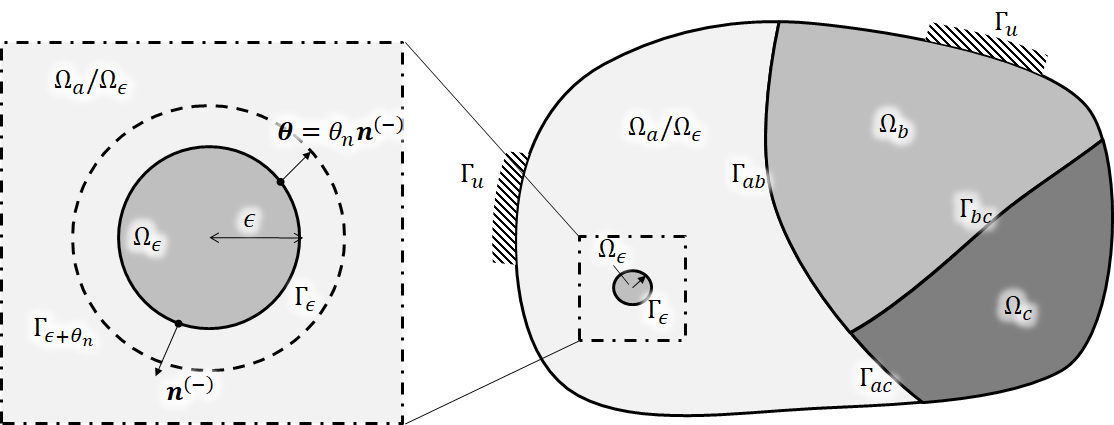
\includegraphics[width=13cm]{./figures/SDforTD.png}
		\caption{Shape derivative for computing the topological derivative}
		\label{fig:TD}
	\end{center}
\end{figure}

$\bm{\theta}$を次式のように設定する.
\begin{align}
	\bm{\theta}=&\theta_{n}\bm{n}^{(-)}	\hspace{1cm}\text{on}\hspace{0.3cm}\Gamma_{\epsilon}\\
	\bm{\theta}=&\bm{0}					\hspace{1.8cm}\text{on}\hspace{0.3cm}\Gamma/\Gamma_{\epsilon}
\end{align}
この時,固有値$\lambda$の形状微分は,\eqref{eq:shape_lambda}に
$\bm{u}=\bm{u}^{\epsilon},\lambda=\lambda^{\epsilon}$を代入することで以下のようになる.
\begin{align}
	&\hspace{0.5cm}D\lambda^{a\rightarrow b}(\Omega_{p\{1\leq p\leq n\}})\cdot\bm{\theta}
	\nonumber
	\\
	=&\int_{\Gamma_\epsilon}(\theta_{n}n_{\gamma}^{(-)}n_{\gamma}^{(-)})
	\Bigr(u_{i,j}^{\epsilon(-)}C_{ijkl}^{b}u_{k,l}^{\epsilon(-)}
	-\lambda^{\epsilon}\rho^{b}u_{i}^{\epsilon(-)}u_{i}^{\epsilon(-)}\Bigl) d\Omega
	\nonumber
	\\
	&+\int_{\Gamma_\epsilon}(\theta_{n}n_{\gamma}^{(-)}n_{\gamma}^{(+)})
	\Bigr(u_{i,j}^{\epsilon(+)}C_{ijkl}^{a}u_{k,l}^{\epsilon(+)}
	-\lambda^{\epsilon}\rho^{a}u_{i}^{\epsilon(+)}u_{i}^{\epsilon(+)}\Bigl) d\Omega
	\nonumber
	\\
	&-\int_{\Gamma_{\epsilon}}(\theta_{n}n_{\gamma}^{(-)}n_{\gamma}^{(-)})
	\Bigr(C_{ijkl}^{b}u_{k,l}^{\epsilon(-)}n_{j}^{(-)}
	-C_{ijkl}^{a}u_{k,l}^{\epsilon(+)}n_{j}^{(+)}\Bigl)
	(u_{i,m}^{\epsilon(-)}n_{m}^{(-)}-u_{i,m}^{\epsilon(+)}n_{m}^{(-)}) d\Gamma
	\nonumber
	\\
	=&\theta_{n}\int_{\Gamma_\epsilon}
	\Bigr(u_{i,j}^{\epsilon(-)}C_{ijkl}^{b}u_{k,l}^{\epsilon(-)}
	-\lambda^{\epsilon}\rho^{b}u_{i}^{\epsilon(-)}u_{i}^{\epsilon(-)}\Bigl) d\Omega
	\nonumber
	\\
	&-\theta_{n}\int_{\Gamma_\epsilon}
	\Bigr(u_{i,j}^{\epsilon(+)}C_{ijkl}^{a}u_{k,l}^{\epsilon(+)}
	-\lambda^{\epsilon}\rho^{a}u_{i}^{\epsilon(+)}u_{i}^{\epsilon(+)}\Bigl) d\Omega
	\nonumber
	\\
	&-\theta_{n}\int_{\Gamma_{\epsilon}}
	\Bigr(C_{ijkl}^{b}u_{k,l}^{\epsilon(-)}n_{j}^{(-)}
	+C_{ijkl}^{a}u_{k,l}^{\epsilon(+)}n_{j}^{(-)}\Bigl)
	(u_{i,m}^{\epsilon(-)}n_{m}^{(-)}-u_{i,m}^{\epsilon(+)}n_{m}^{(-)}) d\Gamma
	\label{eq:SDForTD}
	\\
	=&\theta_{n}\int_{\Gamma_\epsilon}
	\Bigr(e^{\epsilon(-)}:\sigma^{\epsilon(-)}
	-\lambda^{\epsilon}\rho^{b}|\bm{u}^{\epsilon(-)}|^{2}\Bigl) d\Omega
	-\theta_{n}\int_{\Gamma_\epsilon}
		\Bigr(e^{\epsilon(+)}:\sigma^{\epsilon(+)}
		-\lambda^{\epsilon}\rho^{a}|\bm{u}^{\epsilon(+)}|^{2}\Bigl) d\Omega
	\nonumber
	\\
	&-\theta_{n}\int_{\Gamma_{\epsilon}}\Bigl\{
	\Bigr(t_{i}^{\epsilon(-)}+t_{i}^{\epsilon(+)}\Bigl)
		\Bigl(\frac{\partial u_{i}^{\epsilon(-)}}{\partial n}-\frac{\partial u_{i}^{\epsilon(+)}}{\partial n}\Bigr)
	\Bigl\}d\Gamma
	\label{eq:SDForTDRTh}
\end{align}

\begin{figure}[ht]
	\begin{center}
		\includegraphics[height=5cm]{./figures/Rth.png}
		\caption{$(R,\theta)$ coordinate}
		\label{fig:Rth}
	\end{center}
\end{figure}
ここで,
\begin{align}
	x_{1}-z_{1}=R\cos(\theta)
	\nonumber
	\\
	x_{2}-z_{2}=R\sin(\theta)
	\label{eq:xyToRTh}
\end{align}
と座標変換すると$R,\theta$方向の変位は以下のようになる.
\begin{align}
	u_{R}^{\epsilon(-)}(r,\theta)=&\hat{w}_{r}^{(I-)}(\theta)
	+\epsilon\hat{w}_{r}^{(I\hspace{-.15em}I-)}(r,\theta)+O(\epsilon^2)
	\nonumber
	\\
	u_{\theta}^{\epsilon(-)}(r,\theta)=&\hat{w}_{\theta}^{(I-)}(\theta)
	+\epsilon\hat{w}_{\theta}^{(I\hspace{-.15em}I-)}(r,\theta)+O(\epsilon^2)
	\nonumber
	\\
	u_{R}^{\epsilon(+)}(R,r,\theta)=&u_{x_{1}}(\bm{x})\cos(\theta)+u_{x_{2}}(\bm{x})\sin(\theta)
	+\epsilon\hat{w}_{r}^{(I\hspace{-.15em}I+)}(r,\theta)+O(\epsilon^2)
	\nonumber
	\\
	u_{\theta}^{\epsilon(+)}(R,r,\theta)=&-u_{x_{1}}(\bm{x})\sin(\theta)+u_{x_{2}}(\bm{x})\cos(\theta)
	+\epsilon\hat{w}_{\theta}^{(I\hspace{-.15em}I+)}(r,\theta)+O(\epsilon^2)
	\label{eq:SDForTD}
\end{align}
$R=\epsilon r$の関係から,
\begin{align}
	\frac{\partial}{\partial R}=\frac{1}{\epsilon}\frac{\partial}{\partial r}
	\label{eq:RTor}
\end{align}
であることに注意して歪みや応力を計算すると以下のようになる.
\begin{align}
	e_{RR}^{\epsilon(-)}-e_{RR}^{\epsilon(+)}
		=&\frac{\partial u_{R}^{\epsilon(-)}}{\partial n}-\frac{\partial u_{R}^{\epsilon(+)}}{\partial n}
		\nonumber
		\\
		=&2A\bigl\{u_{x_{1},x_{1}}(\bm{z})+u_{x_{2},x_{2}}(\bm{z})\bigr\}
		\nonumber
		\\
		&+(\kappa^{a}-1)B\bigl\{u_{x_{1},x_{1}}(\bm{z})-u_{x_{2},x_{2}}(\bm{z})\bigr\}\cos(2\theta)
		\nonumber
		\\
		&+(\kappa^{a}-1)B\bigl\{u_{x_{1},x_{2}}(\bm{z})+u_{x_{2},x_{1}}(\bm{z})\bigr\}\sin(2\theta)+O(\epsilon)
		\nonumber
		\\
	2\Bigl\{e_{R\theta}^{\epsilon(-)}-e_{R\theta}^{\epsilon(+)}\Bigr\}
		=&\frac{\partial u_{\theta}^{\epsilon(-)}}{\partial n}-\frac{\partial u_{\theta}^{\epsilon(+)}}{\partial n}
		\nonumber
		\\
		=&-\bigl\{u_{x_{1},x_{1}}(\bm{z})-u_{x_{2},x_{2}}(\bm{z})\bigr\}
		\nonumber
		\\
		&-(\kappa^{a}+1)B\bigl\{u_{x_{1},x_{1}}(\bm{z})-u_{x_{2},x_{2}}(\bm{z})\bigr\}\cos(2\theta)
		\nonumber
		\\
		&+(\kappa^{a}+1)B\bigl\{u_{x_{1},x_{2}}(\bm{z})+u_{x_{2},x_{1}}(\bm{z})\bigr\}\sin(2\theta)+O(\epsilon)
		\nonumber
		\\
	e_{\theta\theta}^{\epsilon(-)}=e_{\theta\theta}^{\epsilon(+)}
		=&\frac{(\kappa^{b}-1)}{2}C\bigl\{u_{x_{1},x_{1}}(\bm{z})+u_{x_{2},x_{2}}(\bm{z})\bigr\}
		\nonumber
		\\
		&-\frac{D}{2}\bigl\{u_{x_{1},x_{1}}(\bm{z})-u_{x_{2},x_{2}}(\bm{z})\bigr\}\cos(2\theta)
		\nonumber
		\\
		&-\frac{D}{2}\bigl\{u_{x_{1},x_{2}}(\bm{z})+u_{x_{2},x_{1}}(\bm{z})\bigr\}\sin(2\theta)+O(\epsilon)
		\nonumber
		\\
	\sigma_{RR}^{\epsilon(-)}=\sigma_{RR}^{\epsilon(+)}
		=&2\mu^{b}C\bigl\{u_{x_{1},x_{1}}(\bm{z})+u_{x_{2},x_{2}}(\bm{z})\bigr\}
		\nonumber
		\\
		&+\mu^{b}D\bigl\{u_{x_{1},x_{1}}(\bm{z})-u_{x_{2},x_{2}}(\bm{z})\bigr\}\cos(2\theta)
		\nonumber
		\\
		&+\mu^{b}D\bigl\{u_{x_{1},x_{2}}(\bm{z})+u_{x_{2},x_{1}}(\bm{z})\bigr\}\sin(2\theta)+O(\epsilon)
		\nonumber
		\\
	\sigma_{R\theta}^{\epsilon(-)}=\sigma_{R\theta}^{\epsilon(+)}
		=&-\mu^{b}D\bigl\{u_{x_{1},x_{1}}(\bm{z})-u_{x_{2},x_{2}}(\bm{z})\bigr\}\cos(2\theta)
		\nonumber
		\\
		&+\mu^{b}D\bigl\{u_{x_{1},x_{2}}(\bm{z})+u_{x_{2},x_{1}}(\bm{z})\bigr\}\sin(2\theta)+O(\epsilon)
		\nonumber
		\\
	\sigma_{\theta\theta}^{\epsilon(-)}-\sigma_{\theta\theta}^{\epsilon(+)}
		=&-4\mu^{a}A\bigl\{u_{x_{1},x_{1}}(\bm{z})+u_{x_{2},x_{2}}(\bm{z})\bigr\}
		\nonumber
		\\
		&+4\mu^{a}B\bigl\{u_{x_{1},x_{1}}(\bm{z})-u_{x_{2},x_{2}}(\bm{z})\bigr\}\cos(2\theta)
		\nonumber
		\\
		&+4\mu^{a}B\bigl\{u_{x_{1},x_{2}}(\bm{z})+u_{x_{2},x_{1}}(\bm{z})\bigr\}\sin(2\theta)+O(\epsilon)
	\label{eq:eThThOutEpsSol}
\end{align}
ただし,
\begin{align}
	A=&\frac{\mu^{a}(\kappa^{b}-1)-\mu^{b}(\kappa^{a}-1)}
	{\bigl(\mu^{a}(\kappa^{b}-1)+2\mu^{b}\bigr)(\kappa^{a}-1)}
	\nonumber
	\\
	B=&\frac{\mu^{a}-\mu^{b}}
	{\mu^{a}+\kappa^{a}\mu^{b}}
	\nonumber
	\\
	C=&\frac{\mu^{a}(\kappa^{a}+1)}
	{\bigl(\mu^{a}(\kappa^{b}-1)+2\mu^{b}\bigr)(\kappa^{a}-1)}
	\nonumber
	\\
	D=&\frac{\mu^{a}(\kappa^{a}+1)}
	{\mu^{a}+\kappa^{a}\mu^{b}}
	\label{eq:eThThOutEpsSol}
\end{align}
とおいた.式\eqref{eq:SDForTDRTh}と$\lambda^\epsilon=\lambda+O(\epsilon)$を式\eqref{eq:eThThOutEpsSol}に代入すると,形状微分は以下のようになる
\begin{align}
	&D\lambda^{a\rightarrow b}(\Omega_{p\{1\leq p\leq n\}})\cdot\bm{\theta}
	\nonumber
	\\
	=&\theta_{n}\epsilon\int_{0}^{2\pi}
		\Bigr(\bigl\{e_{RR}^{\epsilon(-)}-e_{RR}^{\epsilon(+)}\bigr\}\sigma_{RR}^{\epsilon(-)}
		+2\bigl\{e_{R\theta}^{\epsilon(-)}-e_{R\theta}^{\epsilon(+)}\bigr\}\sigma_{R\theta}^{\epsilon(-)}
		+e_{\theta\theta}^{\epsilon(-)}\bigl\{\sigma_{\theta\theta}^{\epsilon(-)}-\sigma_{\theta\theta}^{\epsilon(+)}\bigr\}
		\Bigl) d\theta
		\nonumber
		\\
	&-\theta_{n}\epsilon\int_{0}^{2\pi}
		\lambda^{\epsilon}\Bigr(
		\rho^{b}|\bm{u}^{\epsilon(-)}|^{2}-\rho^{a}|\bm{u}^{\epsilon(+)}|^{2}
		\Bigl) d\theta
		\nonumber
		\\
	&-\theta_{n}\epsilon\int_{0}^{2\pi}\Bigr(
		2\bigl\{e_{RR}^{\epsilon(-)}-e_{RR}^{\epsilon(+)}\bigr\}\sigma_{RR}^{\epsilon(-)}
		+4\bigl\{e_{R\theta}^{\epsilon(-)}-e_{R\theta}^{\epsilon(+)}\bigr\}\sigma_{R\theta}^{\epsilon(-)}
		\Bigl) d\theta
	\nonumber
	\\
	=&\theta_{n}\epsilon\int_{0}^{2\pi}
		\Bigr(-\bigl\{e_{RR}^{\epsilon(-)}-e_{RR}^{\epsilon(+)}\bigr\}\sigma_{RR}^{\epsilon(-)}
		-2\bigl\{e_{R\theta}^{\epsilon(-)}-e_{R\theta}^{\epsilon(+)}\bigr\}\sigma_{R\theta}^{\epsilon(-)}
		+e_{\theta\theta}^{\epsilon(-)}\bigl\{\sigma_{\theta\theta}^{\epsilon(-)}-\sigma_{\theta\theta}^{\epsilon(+)}\bigr\}
		\Bigl) d\theta
		\nonumber
		\\
	&-\theta_{n}\epsilon\int_{0}^{2\pi}
		\lambda^{\epsilon}\Bigr(
		\rho^{b}|\bm{u}^{\epsilon(-)}|^{2}-\rho^{a}|\bm{u}^{\epsilon(+)}|^{2}
		\Bigl) d\theta
	\nonumber
	\\
	=&2\pi\epsilon\theta_{n}\Bigl[
	-2\bigl\{\mu^{a}(\kappa^{b}-1)+2\mu^{b}\bigr\}AC
		\bigl\{u_{x_{1},x_{1}}(\bm{z})+u_{x_{2},x_{2}}(\bm{z})\bigr\}^2
		\nonumber
		\\
	&\hspace{1cm}-\bigl(\mu^{b}\kappa^{a}+\mu^{a}\bigr)BD
		\bigl\{u_{x_{1},x_{1}}(\bm{z})-u_{x_{2},x_{2}}(\bm{z})\bigr\}^2
		\nonumber
		\\
	&\hspace{1cm}-\bigl(\mu^{b}\kappa^{a}+\mu^{a}\bigr)BD
		\bigl\{u_{x_{1},x_{2}}(\bm{z})+u_{x_{2},x_{1}}(\bm{z})\bigr\}^2
		\nonumber
		\\
	&\hspace{1cm}-\lambda\Bigr(\rho^{b}-\rho^{a}\Bigl)|\bm{u}(\bm{z})|^{2}
	\Bigr]+O(\epsilon^2)
	\nonumber
	\\
	=&2\pi\epsilon\theta_{n}\Bigl[
	-\frac{2\mu^{a}(\kappa^{a}+1)\Bigl\{\mu^{a}(\kappa^{b}-1)-\mu^{b}(\kappa^{a}-1)\Bigl\}}
			{\bigl(\mu^{a}(\kappa^{b}-1)+2\mu^{b}\bigr)(\kappa^{a}-1)^2}
		\bigl\{u_{x_{1},x_{1}}(\bm{z})+u_{x_{2},x_{2}}(\bm{z})\bigr\}^2
		\nonumber
		\\
	&\hspace{1cm}-\frac{\mu^{a}(\mu^{a}-\mu^{b})(\kappa^{a}+1)}{\mu^{a}+\kappa^{a}\mu^{b}}
		\bigl\{u_{x_{1},x_{1}}(\bm{z})-u_{x_{2},x_{2}}(\bm{z})\bigr\}^2
		\nonumber
		\\
	&\hspace{1cm}-\frac{\mu^{a}(\mu^{a}-\mu^{b})(\kappa^{a}+1)}{\mu^{a}+\kappa^{a}\mu^{b}}
		\bigl\{u_{x_{1},x_{2}}(\bm{z})+u_{x_{2},x_{1}}(\bm{z})\bigr\}^2
		\nonumber
		\\
	&\hspace{1cm}-\lambda\Bigr(\rho^{b}-\rho^{a}\Bigl)|\bm{u}(\bm{z})|^{2}
	\Bigr]+O(\epsilon^2)
	\label{eq:SDForTDRTh}
\end{align}
ゆえに,式\eqref{eq:TSSen}より,トポロジー導関数は以下のように導出される.
\begin{align}
	D_{T}\lambda^{a\rightarrow b}=&\lim_{\epsilon \to 0} \frac{D\lambda^{a\rightarrow b}\cdot\bm{\theta}}{2\pi\epsilon\theta_{n}}
	\nonumber
	\\
	=&\frac{2\mu^{a}(\kappa^{a}+1)\Bigl\{\mu^{b}(\kappa^{a}-1)-\mu^{a}(\kappa^{b}-1)\Bigl\}}
			{\bigl(\mu^{a}(\kappa^{b}-1)+2\mu^{b}\bigr)(\kappa^{a}-1)^2}
		\bigl\{u_{x_{1},x_{1}}(\bm{z})+u_{x_{2},x_{2}}(\bm{z})\bigr\}^2
		\nonumber
		\\
	&+\frac{\mu^{a}(\mu^{b}-\mu^{a})(\kappa^{a}+1)}{\mu^{a}+\kappa^{a}\mu^{b}}
		\bigl\{u_{x_{1},x_{1}}(\bm{z})-u_{x_{2},x_{2}}(\bm{z})\bigr\}^2
		\nonumber
		\\
	&+\frac{\mu^{a}(\mu^{b}-\mu^{a})(\kappa^{a}+1)}{\mu^{a}+\kappa^{a}\mu^{b}}
		\bigl\{u_{x_{1},x_{2}}(\bm{z})+u_{x_{2},x_{1}}(\bm{z})\bigr\}^2
		\nonumber
		\\
	&-\lambda\Bigr(\rho^{b}-\rho^{a}\Bigl)|\bm{u}(\bm{z})|^{2}
	\label{eq:TD}
\end{align}


\end{document}

